%% For double-blind review submission, w/o CCS and ACM Reference (max submission space)
\documentclass[10pt,conference]{ieeetran}%\settopmatter{printfolios=true,printccs=false,printacmref=false}

\usepackage{booktabs}   %% For formal tables:
                        %% http://ctan.org/pkg/booktabs
\usepackage{subcaption} %% For complex figures with subfigures/subcaptions
                        %% http://ctan.org/pkg/subcaption
\usepackage{amsmath,amsthm,amssymb}

\usepackage[table]{xcolor}

\usepackage{threeparttable}

\usepackage{wasysym}

\usepackage{listings}

\usepackage{tikz}

\usepackage{array,multirow}

\usepackage{stmaryrd}

\usepackage[noadjust]{cite}

\usepackage[multiple]{footmisc}

\usepackage[hyphens]{url}

\theoremstyle{definition}
\newtheorem{definition}{Definition}

\newif\ifdraft \drafttrue
\newif\iftext \textfalse
\newif\iflater \latertrue
\newif\ifaftersubmission \aftersubmissionfalse

% !!! PLEASE DON'T CHANGE THESE !!! INSTEAD DEFINE YOUR OWN texdirectives.tex !!!
\makeatletter \@input{texdirectives} \makeatother

%\IEEEoverridecommandlockouts
% The preceding line is only needed to identify funding in the first footnote. If that is unneeded, please comment it out.
\usepackage{cite}
\usepackage{amsmath,amssymb,amsfonts}
\usepackage{algorithmic}
\usepackage{hyperref}
\usepackage{graphicx}
\usepackage{textcomp}
\usepackage[capitalize]{cleveref}
\usepackage[inline]{enumitem}

\usepackage{xcolor}
\newcommand{\bcp}[1]{\ifdraft\textcolor{violet}{{[BCP:~#1]}}\fi}
\newcommand{\leo}[1]{\ifdraft\textcolor{teal}{{[LEO:~#1]}}\fi}
\newcommand{\apt}[1]{\ifdraft\textcolor{blue}{{[APT:~#1]}}\fi}
\newcommand{\rb}[1]{\ifdraft\textcolor{orange}{{[RB:~#1]}}\fi}
\newcommand{\sna}[1]{\ifdraft\textcolor{green}{{[SNA:~#1]}}\fi}
\newcommand{\COQ}[1]{\ifdraft\textcolor{red}{{[COQ DIFFERENCE:~#1]}}\fi}

\usepackage{listings}


\usepackage{xspace}
\newcommand{\cn}{\ifdraft\textsuperscript{\textcolor{blue}{[citation needed]}}\xspace\fi}

\makeatletter
\begingroup
\lccode`\A=`\-
\lccode`\N=`\N
\lccode`\V=`\V
\lowercase{\endgroup\def\memory@noval{ANoValue-}}
\long\def\memory@fiBgb\fi#1#2{\fi}
\long\def\memory@fiTBb\fi#1#2#3{\fi#2}
\newcommand\memory@ifnovalF[1]%>>=
  {%
    \ifx\memory@noval#1%
      \memory@fiBgb
    \fi
    \@firstofone
  }%=<<
\newcommand\memory@ifnovalTF[1]%>>=
  {%
    \ifx\memory@noval#1%
      \memory@fiTBb
    \fi
    \@secondoftwo
  }%=<<
\newcommand\memory@Oarg[2]%>>=
  {%
    \@ifnextchar[{\memory@Oarg@{#2}}{#2{#1}}%
  }%=<<
\long\def\memory@Oarg@#1[#2]%>>=
  {%
    #1{#2}%
  }%=<<
\newcommand*\memory@oarg%>>=
  {%
    \memory@Oarg\memory@noval
  }%=<<
\newcommand*\memory@ifcoloropt%>>=
  {%
    \@ifnextchar[\memory@ifcoloropt@true\memory@ifcoloropt@false
  }%=<<
\long\def\memory@ifcoloropt@true#1\memory@noval#2#3%>>=
  {%
    #2%
  }%=<<
\long\def\memory@ifcoloropt@false#1\memory@noval#2#3%>>=
  {%
    #3%
  }%=<<
\newlength\memory@width
\newlength\memory@height
\setlength\memory@width{23pt}
\setlength\memory@height{14pt}
\newcount\memory@num
\newcommand*\memory@blocks[2]%>>=
  {%
    \memory@num#1\relax
    \fboxsep-\fboxrule
    \memory@ifcoloropt#2\memory@noval
      {\def\memory@color{\textcolor#2}}
      {\def\memory@color{\textcolor{#2}}}%
    \loop
    \ifnum\memory@num>0
      \fbox{\memory@color{\rule{\memory@width}{\memory@height}}}%
      \kern-\fboxrule
      \advance\memory@num\m@ne
    \repeat
  }%=<<
% memory:
%  [#1]: width
%   #2 : count
%  [#3]: height
%   #4 : colour
%  [#5]: label
\newcommand*\memory%>>=
  {%
    \begingroup
    \memory@oarg\memory@a
  }%=<<
\newcommand*\memory@a[2]%>>=
  {%
    % #1 width
    % #2 count
    \memory@ifnovalF{#1}{\memory@width#1\relax}%
    \memory@Oarg\memory@height{\memory@b{#2}}%
  }%=<<
\newcommand*\memory@b[3]%>>=
  {%
    % #1 count
    % #2 height
    % #3 colour
    \memory@ifnovalF{#2}{\memory@height#2\relax}%
    \memory@oarg{\memory@c{#1}{#3}}%
  }%=<<
\newcommand*\memory@c[3]%>>=
  {%
    % #1 count
    % #2 colour
    % #3 label
    \memory@ifnovalTF{#3}
      {\ensuremath{\memory@blocks{#1}{#2}}}
      {\ensuremath{\underbrace{\memory@blocks{#1}{#2}}_{\text{#3}}}}%
    \endgroup
  }%=<<
\makeatother

\newcommand{\judgment}[2]{
  {\centering
  \vspace{\abovedisplayskip}
  \begin{tabular}{c}
    #1 \\
    \hline
    #2
  \end{tabular}
   \vspace{\abovedisplayskip}\par}}

\newcommand{\judgmentbr}[4]{
  {\centering
  \vspace{\abovedisplayskip}
  \begin{tabular}{c}
    #1 \\
    #2 \\
    #3 \\
    \hline
    #4
  \end{tabular}
   \vspace{\abovedisplayskip}\par}}


\newcommand{\judgmenttwo}[3]{
  {\centering
  \vspace{\abovedisplayskip}
  \begin{tabular}{c c}
    #1 & #2 \\
    \hline
    \multicolumn{2}{c}{#3}
  \end{tabular}
  \vspace{\abovedisplayskip}\par}}

\newcommand{\judgmentthree}[4]{
  {\centering
  \vspace{\abovedisplayskip}
  \begin{tabular}{c c c}
    #1 & #2 & #3 \\
    \hline
    \multicolumn{3}{c}{#4}
  \end{tabular}
  \vspace{\abovedisplayskip}\par}}

% Notational conventions
\newcommand{\HIGHSEC}{\textsc{HC}}
\newcommand{\LOWSEC}{\textsc{LC}}
\newcommand{\HIGHINT}{\textsc{HI}}
\newcommand{\LOWINT}{\textsc{LI}}
\newcommand{\IDS}{{\mathcal{I}}}
\newcommand{\ID}{I}
\newcommand{\ME}{\textsc{S}}
\newcommand{\NOTME}{\textsc{O}}
\newcommand{\TRANS}{\ensuremath{-}}
\newcommand{\JAL}{\ensuremath{\mathit{JAL}}}
\newcommand{\ACCYES}{\ensuremath{A}}
\newcommand{\ACCNO}{\ensuremath{I}}
\newcommand{\ACCCODE}{\ensuremath{K}}
\newcommand{\CRCALL}{\ensuremath{\mathit{CALL}}}
\newcommand{\CRRET}{\ensuremath{\mathit{RETURN}}}
\newcommand{\CRBOT}{\ensuremath{\bot}}
\newcommand{\VIS}{\textsc{vis}}
\newcommand{\HID}{\textsc{hid}}
\newcommand{\word}{w}
\newcommand{\addr}{a}
\newcommand{\WORDS}{{\mathcal W}}
\newcommand{\reg}{r}
\newcommand{\REGS}{{\mathcal R}}
\newcommand{\mach}{m}
\newcommand{\machT}{M}
\newcommand{\MACHS}{{\mathcal M}}
\newcommand{\MPT}{\mathit{MP}}
\newcommand{\obs}{o}
\newcommand{\obsT}{O}
\newcommand{\OBSS}{\mathit{Obs}}
\newcommand{\PC}[1]{\PCname(#1)}
\newcommand{\PCname}{\textsc{pc}}
\newcommand{\SP}{\textsc{sp}}
\newcommand{\pol}{p}
\newcommand{\POLS}{\mathcal{P}}
\newcommand{\pinit}{pinit}
\newcommand{\prop}{S}
\newcommand{\contour}{C}
\newcommand{\CONTOURS}{{\mathcal C}}
\newcommand{\component}{k}
\newcommand{\COMPONENTS}{{\mathcal K}}
\newcommand{\trace}{T}
\newcommand{\observer}{O}
\newcommand{\stateobs}{\sigma}
\newcommand{\seq}[1]{\overline{#1}}
\newcommand{\SEQ}[1]{\overline{#1}}
\newcommand{\dstk}[1]{{#1}.\mbox{\it stack}}
\newcommand{\dpcd}[1]{{#1}.\mbox{\it PCdepth}}
\newcommand{\ddep}[2]{{#1}.\mbox{\it depth}({#2})}
\newcommand{\dinit}{\mbox{\it Dinit}}
\newcommand{\empstack}{\mbox{\it empty}}
\newcommand{\access}[2]{\mbox{\it accessible}_{#1}({#2})}
\newcommand{\norm}[1]{\lvert{#1}\rvert}
\newcommand{\MPS}{\mathit{MPState}}
\newcommand{\mpstate}[2]{(#1,#2)}
\newcommand{\mpostate}[3]{(#1,#2,#3)}
\newcommand{\mpstatename}{mp}
\newcommand{\callmap}{cm}
\newcommand{\CALLMAPS}{\mathit{CallMap}}
\newcommand{\ret}[1]{\mathit{justret}\ #1}
\newcommand{\nextPC}{next}
\newcommand{\base}{b}
\newcommand{\stepsto}{\Longrightarrow}
\newcommand{\stepstounder}[1]{\stackrel{\mbox{\tiny{$#1$}}}{\Longrightarrow}}
\newcommand{\stepstounderfull}{\stepstounder{\textsc{RISCV}}}
\newcommand{\manystepsto}{\stepsto^\star}
\newcommand{\obstrace}{\mathit{obstrace}}
\newcommand{\funid}{f}
\newcommand{\FUNIDS}{\mathcal{F}}
\newcommand{\retmap}{\mathit{rm}}
\newcommand{\RETMAPS}{\mathit{RetMap}}
\newcommand{\codemap}{\mathit{fm}}
\newcommand{\CODEMAPS}{\mathit{FuncMap}}
\newcommand{\entmap}{\mathit{em}}
\newcommand{\ENTMAPS}{\mathit{EntryMap}}
\newcommand{\PUT}{\mathit{Until}}
\newcommand{\Trace}{T}
\newcommand{\traceelem}{a}
\newcommand{\TRACEELEMS}{A}
\newcommand{\head}{\mathit{head}}
\newcommand{\last}{\mathit{last}}

\newcommand{\stepstoobs}[1]{\xrightarrow{#1}}
\newcommand{\polstep}{\rightharpoonup}
\newcommand{\stepstopol}[1]{\overset{#1}{\rightharpoonup}}
%\newcommand{\stepstopol}[1]{\overset{#1}{\rightharpoonup}_P}

\newcommand{\stepplus}{\Rightarrow}
\newcommand{\stepkappa}{\Rightarrow_\kappa}
\newcommand{\induced}[2]{(#1, #2)^*}
\newcommand{\flows}{\sqsubseteq}
\newcommand{\flowsstrict}{\sqsubset}
\newcommand{\initmach}{\MACHS_{\mathit{init}}}
\newcommand{\initcontour}{\CONTOURS_{\mathit{init}}}
\newcommand{\closure}[1]{\textit{Close}#1}
\newcommand{\variant}[2]{\textit{Vars}(#1, #2)}
\newcommand{\isinf}{\mathit{inf}}

\newcommand{\Last}[1]{\mathit{Last}(#1)}

\newcommand{\HALT}{\textsc{HALT}}

\newcommand{\underscore}{\mbox{\_}}

\newcommand{\propdef}[1]{\text{\sc #1}}

\newcommand{\TRACE}[1]{\mathit{Trace}~(#1)}
\newcommand{\MTRACE}{\TRACE{\MACHS}}
\newcommand{\MOTRACE}{\TRACE{\MACHS \times \OBSS}}
\newcommand{\MPOTRACE}{\TRACE{\MACHS \times \POLS \times \OBSS}}


\makeatletter
\newcommand{\linebreakand}{%
  \end{@IEEEauthorhalign}
  \hfill\mbox{}\par
  \mbox{}\hfill\begin{@IEEEauthorhalign}
}
\makeatother

\begin{document}

%% Title information
\title{Formalizing Stack Safety as a Security Property}

\author{
  \IEEEauthorblockN{
    Sean Noble Anderson
  }
  \IEEEauthorblockA{
    Portland State University\\
    ander28@pdx.edu\\
  }
  \and
  \IEEEauthorblockN{
    Leonidas Lampropoulos
  }
  \IEEEauthorblockA{
    University of Maryland, College Park\\
    leonidas@umd.edu\\
  }
  \and
  \IEEEauthorblockN{
    Roberto Blanco
  }
  \IEEEauthorblockA{
    Max Planck Institute for Security and Privacy\\
    roberto.blanco@mpi-sp.org\\
  }
  \linebreakand
  \IEEEauthorblockN{
    Benjamin C. Pierce
  }
  \IEEEauthorblockA{
    University of Pennsylvania\\
    bcpierce@cis.upenn.edu\\
   }
  \and
  \IEEEauthorblockN{
    Andrew Tolmach
  }
  \IEEEauthorblockA{
    Portland State University\\
    tolmach@pdx.edu\\
  }
}

%% Keywords
%% comma separated list
\ifcameraready
\keywords{Stack Safety, Micro-Policies}  %% \keywords are mandatory in final camera-ready submission
\fi

\maketitle

\begin{abstract}

The term {\em stack safety} is associated with a
variety of compiler, run-time, and hardware mechanisms for protecting stack
memory. But, unlike ``the heap,'' the stack does not correspond to a single
high-level language concept. Rather, it corresponds to the fundamental
abstraction of functions, in all of the forms that they can take.
The protean nature of the functional abstraction makes stack safety
difficult to specify.

We propose a formal characterization of stack safety based on
concepts from language-based security. Stack safety is decomposed
into an integrity property and a confidentiality property for each
of the caller and the callee, as well as a control-flow property.

Our motivating enforcement mechanism,
the ``lazy'' stack safety micro-policies proposed by
Roessler and DeHon~\cite{DBLP:conf/sp/RoesslerD18}, permit functions
to write into one another's frames, but taint the result so that the frame's
owner cannot access it. No existing characterization of stack safety
captures this style of safety. We capture it by defining the properties in
terms of the observable behavior of the system.

The stack interacts with a large number of language features that are often excluded
from discussion of stack safety. Our properties support a system with
both caller- and callee-saved registers, arguments passed on the stack,
tail-call elimination, \ifexceptions exceptions \fi. They are modular by
design, in order to be further extensible to other features.

We validate our properties by using them to distinguish correct implementations
of Roessler and DeHon's micro-policies from incorrect ones
via property-based random testing. Our testing successfully detects violations
in several broken variants, including Roessler and DeHon's original lazy policy.
A fixed version of the policy does pass our tests.

\end{abstract}

\newcommand{\paragraphx}[1]{\emph{#1.}}

\section{Introduction}

\rb{\textbf{The call stack and its security.} Maybe a few opening words to set
  the stage and bring two things to the front: (1) functions and subroutines as
  fundamental building blocks of any kind of structured programming; and (2) the
  stack as the natural abstraction to manage these in a computer. And also maybe
  a little bit more about the width, the gravity and the \emph{foundational
  nature} of attacks on the stack, which the sentence below touches on
  summarily.}
%
The call stack is a perennial target for low-level attacks, leading to
dire consequences from leakage and corruption of private stack data
to control-flow hijacking.
%
\rb{We can mention things like e.g. the most recent CWE Top 25 Most Dangerous
    Software Weaknesses from MITRE, cf.
    \url{https://cwe.mitre.org/top25/archive/2022/2022_cwe_top25.html}, where
    e.g. \#1 (Out-of-bounds Write), \#5 (Out-of-bounds Read) and \#7 (Use After
    Free), that is a good number of the most important and prevalent
    vulnerability types are closely related to the stack. These will show up in
    other popular rankings as well.}
%
To foil such attacks, a menagerie of
software and hardware protections have been proposed,
%
including stack canaries~\cite{Cowan+98},
bounds checking~\cite{NagarakatteZMZ09,NagarakatteZMZ10,DeviettiBMZ08},
split stacks~\cite{Kuznetsov+14},
shadow stacks~\cite{Dang+15,Shanbhogue+19},
capabilities~\cite{Woodruff+14,Chisnall+15,SkorstengaardLocal,SkorstengaardSTKJFP,Georges+21},
and hardware tagging~\cite{DBLP:conf/sp/RoesslerD18}.
  \ifaftersubmission\apt{Mostly from
  nick; there could be more}\bcp{Yes, going back to MIT days---we should
  include several more of these, if only to give readers the impression that
this is a well-studied mechanism (so formalizing its protections is
useful).}
\fi
%
\rb{Did we want to add even more techniques? Is this selection broad enough?
  Anyway reference that we'll be looking at these more closely later.}

The protections offered by such mechanisms are commonly described by giving
concrete examples of attacks that they can prevent---corruption of return
addresses, buffer overflows, use of uninitialized variables, etc.---leaving
a more formal characterization to the reader's intuition.
%
\rb{Begins to anticipate subsequent discussion. This is even something of an
  understatement: some papers (esp. newer ones?), make concrete claims, though
  they remain informal. Arguably, none have a truly formal characterization in
  mind (with the qualified exception of \cite{SkorstengaardSTKJFP}): this is one
  of the novelties of this work!}
%
Previous attempts
to produce a formal characterization do so using a {\it fully abstract overlay semantics},
a style of correct-by-construction machine \cite{SkorstengaardSTKJFP}.
But this approach is not suitable for the {\em lazy} enforcement mechanism
of Roessler and DeHon, in which stores are not checked, and illegal stores are
only caught when their location is later read. We aim to provide a stack-safety
property suitable for testing lazy enforcement.
%
\rb{Need to discuss overlay semantics, but also note that it is very intensional
  and very specific, as the authors acknowledge. I'd introduce this a bit more
  gradually. Also, if phrased this way, it sounds like its main drawback is a
  lack of generality, to which we should contrast a more general approach, not
  just one that is specialized to a specific policy, i.e. lazy micro-policies
  (I'd try to present these more gradually as well).}

We propose a novel characterization of stack safety using the formal tools of language-based
security~\cite{sabelfeld2003language}, decomposing stack safety into
the {\em integrity} and {\em confidentiality} of the caller’s local state
and the callee's behavior during the callee's execution, plus the control flow protection
of {\em well-bracketed control flow}~\cite{SkorstengaardSTKJFP} (\(\wbcf\)).
\ifexceptions
We also extend WBCF to a setting with exceptions,
in which there may be multiple points at which a callee can ``return.''
\fi
%
\rb{Connect this to the shortcomings of previous work. I'd give at least a quick
  explanation of what the various properties roughly entail in practice (e.g.,
  secrecy of private data, etc.). The comment about the single extension of
  exceptions seems disconnected from the rest.}

This gives us a total of five core properties: \(\wbcf\)
caller integrity (\(\clri\)), caller confidentiality (\(\clrc\)),
callee integrity (\(\clei\)), and callee confidentiality (\(\clec\)).

To demonstrate the utility of our formal characterization, we use these
properties to validate and improve an existing enforcement mechanism, the
{\em stack safety micro-policies} of Roessler and DeHon~\cite{DBLP:conf/sp/RoesslerD18}, re-implemented
in the Coq proof assistant on top of a \rb{formal} RISC-V specification.  We
use QuickChick~\cite{Denes:VSL2014,Pierce:SF4}, a property-based testing
tool for Coq, to generate random programs and check
that Roessler and DeHon's micro-policies correctly detect the ones that
attempt to violate one of our properties. Furthermore, we
check that the testing framework is able to generate counterexamples
that violate our properties but are \emph{not} halted by incorrect
variants of the enforcement mechanisms, including ones that we accidentally created
while implementating the micro-policy and ones that we
intentionally crafted to increase our confidence in the effectiveness
of our testing.
%
\rb{This and the following paragraph could start more generally (we need to
  answer the question of why these experiments, what is their interest), and
  probably motivate the use of PBT (experiment results below show there's
  benefit in them!) and, somewhere at least, talk about other points in the
  spectrum.}

We find that Roessler and DeHon's \emph{Lazy Tagging and Clearing}
violates the temporal aspect of confidentiality in
cases where data can leak across repeated calls to the same callee,
and also violates integrity if the leak uses the caller's frame. We
propose a variant of {\em Lazy Tagging and Clearing} that testably enforces
confidentiality, albeit at some performance cost.
%
\rb{Anything to add from personal communications? More details later? Shows
  these things are very hard to get right -- like the latest work on Cerise,
  also motivated by this very work.}

\subsection{Motivation}

Security mechanisms designed to prevent a certain attack can be brittle---successfully
eliminating the attack as it exists at the time of publication, but leaving room for attackers
to find new, similar attacks. To mitigate this risk, mechanisms should aim to enforce formal
properties of correct behavior that can be proven or tested. Such properties become the
specification against which enforcement can be validated; even enforcement mechanisms that do
not fulfill the property benefit from the ability to articulate {\it why} they fail.
%
\rb{Good stuff! There is some overlap between this discussion and the opening
  motivation, maybe we could restructure things a bit so that those threads are
  unified?}

Stack safety is challenging to specify in full generality, because the stack is fundamentally
an architecture-specific construct. (Contrast Acevedo de Amorim et al.'s \cite{} work on heap safety,
which is broadly consistent across architectures and language semantics, and therefore amenable
to a very general approach.)
The desired behavior of the stack varies based on ISA, calling convention,
and the features of whichever programming language originated the code.
For instance, the current state-of-the-art stack-safety specification from Georges et al.
\cite{Georges22:TempsDesCerises} supposes a machine with only straightforward call-and-return
control flow, and therefore defines {\it Well-bracketed Control Flow} (WBCF) under the assumption that
a callee should always return to its caller. But, in the presence of tail-call elimination, a
return from a callee to a distant ancestor is perfectly reasonable. Any addition of new features
must be accompanied by tweaks to the model.
%
\rb{This point is extremely important!}

We are not attempting to create a universal definition of stack safety for all systems.
Rather, we define the stack safety of a single, fairly realistic system, decomposed into
(1) a lightweight model of the system and its security-relevant features, from which we
derive the integrity, confidentiality, and control-flow requirements of each call and
return, (2) the application of that model to a particular target system, and (3)
the formal criteria for integrity, confidentiality, and control flow
to obey the requirements. We consider the criteria in (3) to represent universal definitions
that are parameterized by (1).
%
\rb{Sharpen, contrast the universal definitions (or a framework of parametric
  definitions, say) with the concrete instance we study, again with its interest
  properly motivated.}

We treat stack safety as multiple properties, rather than one multi-faceted property, because
not all enforcement mechanisms attempt to implement all aspects of stack safety. Some focus
exclusively on control flow, some enforce integrity but not confidentiality, and many
focus on the caller over the callee.
%
\rb{Also sharpen after extended discussion?}

\paragraph*{Permissiveness, Laziness, and Tagged Architectures}

Security properties tend to be conservative, identifying violations that would be
harmless in practice. But enforcement mechanisms make trade-offs in the name of performance
and of compatibility with existing codebases. In a crucial motivating example for this work,
Roessler and DeHon \cite{} present a collection of tag-based enforcement mechanisms
using PIPE \cite{???}, a tagged hardware reference monitor. In monitors such as PIPE and
STAR \cite{???}, every value in memory and registers is paired with a {\em metadata tag}.
A set of software-defined rules, termed a micro-policy, determines the tags for operation
results based on the tags of their inputs---or, if the input tags are in a dangerous
combination, it may halt the machine (a ``failstop.'')

Roessler and DeHon find that the intuitive way to enforce stack safety in this setting
is inefficient when allocating and clearing stack frames, because each word must be initialized
with a tag corresponding to the (depth of the) current function activation. They propose
{\em Lazy Tagging and Clearing}, in which tags are not initialized at allocation, but only
when a function writes to memory. This means that writes cannot be prevented, necessarily
violating existing models of stack safety. Instead the micro-policy enforces that memory be
read by the same fuction that wrote it. The owner of the data will never see the changes,
so it is secure in the sense that the attacker is unsuccessful at changing program behavior
(except, perhaps, by causing a fault.) We elaborate that sense, and test whether the
micro-policy fulfills it.

This key motivation leads us to present integrity and confidentiality as predicates on (pairs of)
machine states that make claims about the future observable behavior of execution from those states.
That is not to say that our properties are specialized for lazy micro-policies. It also supports
normal ``eager'' micro-policies, and should support other enforcement mechanisms. In fact, \(\clri\)
and \(\clrc\) are even weaker than necessary to support Roessler and Dehon's micro-policy,
while \(\clec\) and \(\clei\) are stronger properties that they do not attempt to enforce.
%
\rb{Does this discussion (at least in part) belong in the general background
  section, some even in key ideas? It still feels a little out of order to me,
  and occasionally too detailed for the introduction?}

\rb{\textbf{A menagerie of protection mechanisms.}
%
We have made explicit the key point that there is \emph{not} a single stack
abstraction. This paves the way for a \emph{general} idea of stack protection
that is widely applicable with high-level concepts that remain unchanged (and I
think it's particularly important to at least introduce these more immutable
parts early on). The fact that this general ``framework'' requires low-level or
specific specializations is a predictable consequence of the protean nature of
the call stack.
%
\\
%
Let us return to a selection of representative policies in our menagerie and
consider how they fit into the framework. At the highest level, we can classify
all those techniques into two large groups, software-based and hardware-based.
Traditionally, most practical protections are implemented in software, so we
start by considering this first group.
%
\\
%
We can make two general observations about these software based techniques.
Firstly, (as we will see: discussion? technical details?) these techniques are
\emph{less modular} than their hardware counterparts. That is, the
countermeasures are tightly coupled with the program code they protect, and
consequently more effort is required to disentangle the program from the
protections, and to understand the impact of the latter on the former. This is
true of any systematic attempt to study the security of stack protection
policies, including their adaptation to our framework. (Owing to this added
complexity, software policies will not be the cleanest or most elegant exemplars
of use of the framework, its salient features and practical utility; this partly
motivates the focus on hardware policies.)
%
\\
%
(The above remark holds \emph{at least in a ``single-level model''} that
considers assembly language/machine code programs. In general, (low-level)
protections are introduced by a compiler or similar tool. One could consider a
multi-level extension of the framework pairing models of high-level programs and
the security transformations performed by a (stack-secure) compiler.)
%
\\
%
Secondly, the guarantees generally offered by software-based policies are
\emph{less absolute}, being defined more or less informally and usually
providing few definite guarantees of absence of \emph{general} classes of
errors. (The following discussion elaborates on this. It is conceivable that an
extended and more sophisticated framework could add \emph{probabilistic
reasoning} capabilities to capture and reason about the effects of less strict
protection mechanisms. This would be another orthogonal development to what is
presented here. In this paper, we are interested in assessing the complete
\emph{absence} of broad classes of vulnerabilities --- modulo any modeling gaps
or defects. In passing, this would extend the security properties to e.g. larger
system verification efforts.)
%
\\
%
One by one, consider the following specimens of software protection mechanisms
(quick explanations inlined?):
%
\\
%
\begin{itemize}
%
\item \emph{Stack canaries}. The purpose of canaries is to \emph{increase} the
  difficulty of some attacks on the stack, usually (always?) buffer overflows.
  They can never provide any absolute security guarantees and therefore do not
  satisfy any of our properties (some of the properties, e.g. confidentiality,
  are completely out of scope.) Although tedious, we could we could model this
  mechanism in our framework with the appropriate adaptations --- and
  unsurprisingly, testing would find property violations, which we already know
  are there: the results of this effort would be unsurprising and not as useful
  or instructive as other experiments.
%
\item \emph{Bounds checking}. This is fundamentally a high-level technique, even
  more obviously so than stack canaries (which could still detect violations
  caused by external code). Bounds checking only applies to code that has been
  instrumented by the ``secure compiler'' (i.e., to whole programs); it does not
  impose any constraints on adversarial code. The attacker model is therefore
  rather weak. (Certain variants, like SoftBound, are good targets for lifting
  our framework to the source level by e.g. using a C-language semantics and
  using Tagged C for security modeling; the lifted versions of our properties
  would likely hold under the expected assumptions. HardBound is probably an
  interesting transitional case because it uses capability-like hardware
  primitives for enforcement; it could be close to ongoing and future work to
  verify stack safety on capability machines, e.g. based on Cerise -- discuss
  together?)
%
\item \emph{Shadow stacks}. Like stack canaries, shadow stacks are
  ``probabilistic techniques'' in that they ``restrict the flexibility available
  in creating gadget chains'' (Shanbhogue et al.). This technique is solely
  concerned with control-flow integrity, and so closely related to our
  well-bracketed control flow. Nevertheless, and again, it is only an
  approximate technique, and our testing framework would be able to find the
  expected attacks against our security property.
%
\item \emph{Split stacks}. The security claims of split stacks are stronger than
  those of most software countermeasures, i.e., they are meant to guarantee
  their titular code-pointer integrity. They explicitly offer no protections on
  stack data (i.e., integrity and confidentiality), and so restrict themselves
  to well-bracketed control flow. (This is probably closer to our framework than
  most other software techniques, and it seems like it would be easier to model
  as well. However, this is again work based on high-level languages and would
  benefit from a higher level of abstraction.)
%
\item \ldots
%
\end{itemize}
%
Opposed to the above group of software techniques we have hardware-based
protection policies (more in background/technical preliminaries?). Although
programs must effectively leverage the protection mechanisms offered by the
hardware, the distinction between those protections and the program logic itself
is much cleaner: it is fairly simple to separate the use of the security
features in the hardware (and their effects in program code) from regular
program code. They also tend to aspire to offer complete protection against
entire classes of attacks. Both aspects make this family of techniques a better
fit for illustrating and showcasing our techniques.
%
\\
%
Why favor micro-policies? Their design is more flexible and arguably more
general than capability machines (of course, they pay a performance price for
this). This generality and ease of programming make them good candidates for an
exploration the design space of stack protection policies and proof of concept
implementations. On the practical side, there is a number of existing policies
available to examine (not just lazy policies!) --- and we find how they satisfy
our properties, how they do not, and errors in some of them, and see how to
correct them. Lazy enforcement is particularly novel, but not the only
possibility. This additional breadth is beneficial for the proof of concept
stage.
%
\\
%
Regarding capability machines, we know that most designs based on capability
machines do not satisfy our properties (or do so incurring significant costs),
and that fixes are not trivial and involve new types of capabilities (in a
sense, are they any more ``realistic?'' Only the latest Cerise paper would seem
to satisfy our properties, is directly influenced by previous versions of this
work, and is a reasonable target for ongoing/further study -- but this is not
easy, and even the author(s) estimate it would be a significant amount of work,
especially full proofs (references, communications, etc.).
%
\\
%
\ldots
%
}

\subsection{Contributions}

In sum, we offer the following contributions:

\begin{itemize}
\item We formalize permissive stack confidentiality and integrity properties,
  which are parameterized over a notion of external
  observation, and are violated only if accessing secrets or overwriting
  data causes a visible change in system behavior.
\item We instantiate these definitions with a realistic
  system with features such as argument passing
  on the stack, callee-saves registers, and tail-call elimination.
  Our model is modular enough that adding these features is straightforward.
\item Our formalization of well-bracketed control flow in the presence of tail-call
  elimination \ifexceptions and exceptions \fi is a novelty over existing models.
\item We use property-based random testing to validate the relationship between
  our properties and micro-policies.
\end{itemize}

Our artifact contains Coq formalizations of our properties for illustrative purposes
as well as their testing implementation. There are no proofs---we use primarily Coq for the
QuickChick library and to ensure that the formalizations are unambiguous.
%
\rb{Will have another look after the full pass.}

\paragraph*{Limitations}

%Our concurrency model is fairly
%simplistic, assuming a fixed number of threads each with its own dedicated processor.
We model memory-safe stack objects, but not a heap. Regions outside of
stacks can be used however the compiler likes, including as a heap, but no protection is
built in and our properties assume that if a pointer to a stack object is stored there,
it is permanently compromised.

Our properties are termination insensitive: in order to support enforcement mechanisms
that failstop rather than execute dangerous code, the properties must treat failstops
as invisible to the attacker. We extend this insensitivity to all errors for simplicity.
This is consistent with our treatment of properties that specify the state after a return,
in that a callee that diverges for any reason will never reach the return, and will fulfill
the property vacuously.
%
\rb{Limitations in the introduction or later? Orthogonality of the heap, morally
  similar interesting setups on the stack? Termination sensitivity and
  capability machine semantics?}


\section{Key Ideas}
\label{sec:ideas}

The paper is structured as follows. In \cref{sec:example}, we will walk through a function
call in a simple example machine and discuss how each of our properties applies to it,
informally. In the process we discuss some motivation for the properties, from a security
perspective: we consider a simple attacker, and discuss the harm that it can do to
its caller. This perspective is essential to understanding how lazy enforcement can
be safe: even if an attacker can overwrite some memory, if it cannot accomplish
its bigger-picture goals, the system is safe.

Then in \cref{sec:machine} we will introduce the machine model that we test, and give
its {\em security semantics}, described in brief below. We formalize the definitions of
stack safety that derive from the security semantics in \cref{sec:props}.
\Cref{sec:testing} describes the testing framework, and
\cref{sec:relwork,sec:future} discuss related and future work.
The remainder of this section introduces ideas that will be important throughout.

\paragraph*{Security Semantics and Property Structure}

A {\it security semantics} extends a machine
with additional context about the identity of current and pending
functions (which act as security principals) and about the registers and memory they require
to be secure. This added context is purely notional;
it does not affect the real machine. The security context
evolves dynamically through the execution of {\it security-relevant operations},
which include events like calls, returns, and frame manipulations.
Our security properties are phrased in terms of this context, often as predicates
on future states, e.g. of the form ``when control returns to the current function...'',
or relations on traces of future execution (hyper-properties).

The security-relevant operations typically correspond to underling machine instructions,
but the correspondence may not be obvious just by inspecting the machine code.
For example, in the tagged RISC-V machine we use in our examples and tests,
calls and returns are conventionally performed by {\tt jal} (``jump-and-link'')
and {\tt jalr} (``jump-and-link-register'') instructions, respectively, but these
instructions might also be used for other things. An instantiation of an operation
might require some external mechanism for distinguishing which instructions are
security-relevant; the most obvious technique is to add optional labels to instructions,
but the theory does not depend on this choice.

Whatever the mechanism for labeling transitions, we get a base
machine transition \(\mach \xrightarrow{\bar{\psi}, \obs} \mach'\), where \(\obs\) is
an event (see below) and \(\bar{\psi}\) is a list of security-relevant operations.
We then lift this into a transition between pairs of machine states and contexts,
\((\mach,\context) \stepstounder{\overline{\psi},\obs} (\mach', \context')\).

The set of security-relevant operations (\(\Psi\)) covered in this paper is given in
\cref{tab:psi}. Those that we explore in detail in \cref{sec:example}
are shown in white: calls, returns, and the allocation and deallocation of local memory.
In \cref{sec:machine}), we cover additional operations that add parameters to the examples',
to support various forms of memory sharing \ifexceptions , exceptions, \fi
and tail-call elimination. These are shown in light gray.
We give a proof-of-concept formalization of a more sophisticated, heap-like sharing model
based on pointer provenance in \cref{app:ptr}, represented by the dark grey
operations, but we do not test this.

\newcommand{\example}{\rowcolor{black!0}}
\newcommand{\testing}{\rowcolor{black!10}}
\newcommand{\theory}{\rowcolor{black!25}}

\begin{table}
  \begin{tabular}{| l | l |}
    \hline
    \(\psi \in \Psi\) & Parameters \\
    \hline
    \example \(\mathbf{call}\) & Target address, argument registers \\
    \testing & Stack argument offset \& size \\
    \example \(\mathbf{return}\) & \\
    \example \(\mathbf{alloc}\) & Offset \& size \\
    \testing & Public flag \\
    \example \(\mathbf{dealloc}\) & Offset \& size \\
    \testing \(\mathbf{tailcall}\) & As \(\mathbf{call}\) \\
    \hline
    \multicolumn{2}{|c|}{{\it Pointer provenance operations}} \\
    \hline
    \theory \(\mathbf{promote}\) & Register, offset \& size \\
    \theory \(\mathbf{propagate}\) & Source register/address \\
    \theory & Destination register/address \\
    \theory \(\mathbf{clear}\) & Target register/address \\
    \hline
  \end{tabular}
  \caption{Security-relevant Operations and their Parameters}
  \label{tab:psi}
\end{table}

Our security semantics has similarities to the overlay semantics that have been proposed
to characterize stack safety in the past~\cite{SkorstengaardSTK}, but it does not restrict
the behavior of the underlying machine in any way. Rather, it tracks additional context
about the history of security-relevant operations, which inform the criterion a machine
must satisfy in order to correctly obey the properties.

The security principals in our account of stack safety are function
activations: at any given time, pending activations
have security requirements that are recorded in a call stack, and the current
activation tracks context information that will inform its requirements when
it makes a call. Each activation has a {\it view}
of the system that maps each state element to a {\it security class}:
it may be private to an inactive principal (\(\sealed\)),
in an allocated object that is accessible to the current principal (\(\object\)),
available to be allocated (\(\unsealed\)), or
always accessible (\(\public\)).

\paragraph*{Events}

It is common to specify the behavior of a system, including security properties, in
terms of traces of observable {\em events} rather than details of the machine state.
Lazy enforcement works because the deferred check catches errors before they appear
in the trace. The nature of events is a parameter of the machine, and can be specialized
to any notion of observable behavior.

\paragraph*{Variants and Non-interference}

To characterize confidentiality, we borrow the idea of \emph{variant} states
from the theory of non-interference. Non-interference is a way of expressing
the flow of information through the system. If we begin with a state \(\mach\)
and modify it to \(\nach = \mach[\component \mapsto v]\) for arbitrary \(v\),
then execute both \(\mach\) and \(\nach\), any differences in the outputs they
produce must be the result of accessing \(\component\).

\paragraph*{Putting It Together}

Putting these ideas together, we get the basic structure of a property in our model.
First we define the security-relevant operations that we support, a security context,
and the function according to which the security context updates with each step.
Then, we define a predicate on states and contexts that expresses the requirements
for our security property, using variants, assertions about future states, and comparison
of event traces. Finally, in order to apply the property to a specific machine, we
must determine how the machine's execution translates into security relevant operations.


\section{Properties by Example}
\label{sec:example}

In this section we consider a simple setting with calls, returns, and private allocations,
on a RISC-V machine with a PIPE tagging system. In this system a value is a pair of a
word (the ``payload'') and a tag drawn from some set \(\mathcal{T}\).
%\(\mathcal{V} ::= \mathcal{W} \times \mathcal{T}\),
%for some type  of tags to be elaborated later, with \(|(w,t)| = w\).
Figure \ref{fig:RISCVregs} gives an example division of the RISC-V registers into
security classes.
Figure \ref{fig:main} gives the C code and corresponding compiled RISC-V code
for a function {\tt main}. Code is compiled using the standard RISC-V
calling conventions~\cite{??}; the stack grows towards lower addresses. We assume that
{\tt main} begins at address 0 and its callee {\tt f} at address 100.

{\tt main} takes a secret as its argument and initializes a variable to contain
potentially sensitive data. We define an observable event to be a store
to a special address, called {\tt out}.
{\tt main} calls another function {\tt f},
and afterward may decide to output its secret based on the contents of
its sensitive data. In this case, since {\tt sensitive} is initialized to 0,
it should not---instead it will output the results of {\tt f}.

\begin{figure}
  \begin{subfigure}{\columnwidth}
    {\tt
      volatile int out;

      void main(int secret) \{

      ~ ~ int sensitive = 0;

      ~ ~ int res = f();

      ~ ~ if (sensitive == 42)

      ~ ~ ~ ~ out = secret;

      ~ ~ else

      ~ ~ ~ ~ out = res;

      \}}
  \end{subfigure}
  \begin{subfigure}{\columnwidth}
    \begin{tabular}{r l | l}
      \labeledrow{0:}{addi sp,sp,-20}{\(\mathbf{alloc} ~ (-20,20)\)}
      \labeledrow{4:}{sd ra,12(sp)}{}
      \labeledrow{8:}{sw a1,8(sp)}{}
      \labeledrow{12:}{sw zero,4(sp)}{}
      \labeledrow{16:}{jal f,ra}{\(\mathbf{call} ~ \mathtt{f} ~ \emplist ~ \emplist\)}
      \labeledrow{20:}{sw a0,0(sp)}{}
      \labeledrow{24:}{lw a4,4(sp)}{}
      \labeledrow{28:}{li a5,42}{}
      \labeledrow{32:}{bne a4,a5,L1}{}
      \labeledrow{36:}{lw a0,8(sp)}{}
      \labeledrow{40:}{sw a0,out}{}
      \labeledrow{44:}{j L2:}{}
      \labeledrow{L1, 48:}{lw a0,0(sp)}{}
      \labeledrow{52:}{sw a0,out}{}
      \labeledrow{L2, 56:}{ld ra,12(sp)}{}
      \labeledrow{60:}{addi sp,sp,20}{\(\mathbf{dealloc} ~ (0,20)\)}
      \labeledrow{64:}{jalr ra}{\(\mathbf{return}\)}
    \end{tabular}
  \end{subfigure}
  \begin{subfigure}{\columnwidth}
    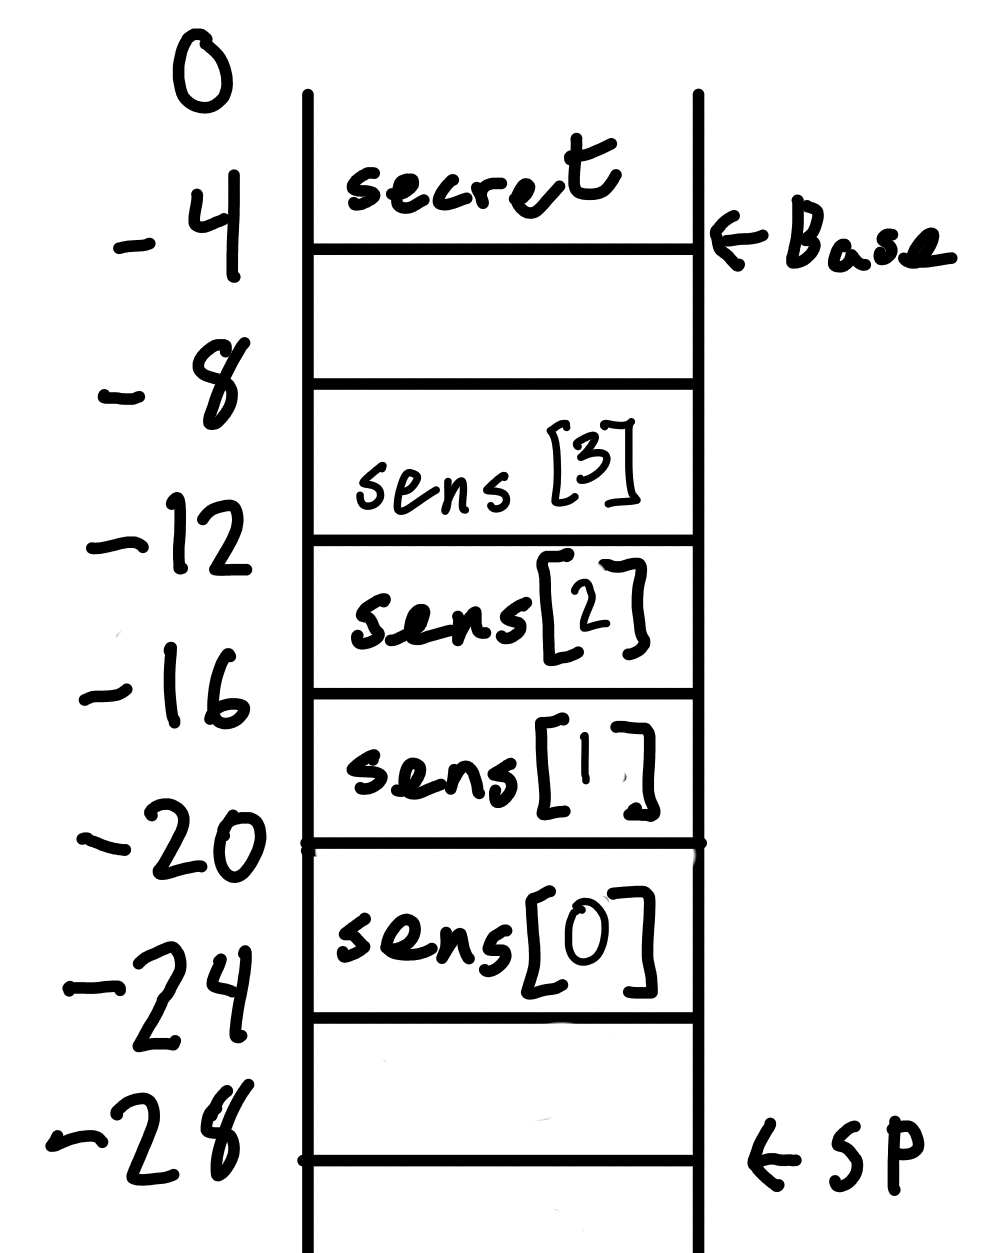
\includegraphics[width=\columnwidth]{stacklayout.png}
  \end{subfigure}

\caption{Example: Main}
\label{fig:main}
\end{figure}

Suppose that {\tt f} is actually an attacker seeking
to leak {\tt secret}. It might do so in a number of ways, shown as snippets of
assembly code in Figure \ref{fig:f}.
%
In Figure \ref{subfig:direct}, {\tt f} takes an offset from the stack
pointer, accesses {\tt secret}, and directly outputs it. But more
subtly, even if somehow prevented from outputting {\tt secret} directly, {\tt f}
can instead return that value so that {\tt main} stores it to {\tt out},
as in Figure \ref{subfig:indirect}.
%
Beyond simply reading {\tt secret}, the attacker might overwrite {\tt sensitive}
with 42, guaranteeing that {\tt main} publishes its own secret unintentionally
(Figure \ref{subfig:integrity}).
Attacks of this kind do not violate {\tt main}'s confidentiality, but
rather its {\it integrity}.
In Figure \ref{subfig:WBCF}, the attacker arranges to return to the
wrong instruction, thereby bypassing the check and publishing {\tt secret} regardless,
violating the program's {\it well-bracketed control flow} (WBCF.)
%
In Figure \ref{subfig:WBCF2}, a different attack violates WBCF, this time
by returning to the correct program counter but with the wrong stack pointer.
\footnote{We pad the last two variants with {\tt nop}s just so that all the
snippets have the same length, which simplifies some later explanations.}

\begin{figure}
  \begin{subfigure}[b]{\columnwidth}
    \vspace{\abovedisplayskip}
    \begin{tabular}{r l | l}
      \labeledrow{100:}{lw a4,8(sp)}{}
      \labeledrow{104:}{sw a4,out}{}
      \labeledrow{108:}{li a0,1}{}
      \labeledrow{112:}{jalr ra}{\(\mathbf{return}\)}
    \end{tabular}
    \caption{Leaking {\tt secret} directly}
    \label{subfig:direct}
  \end{subfigure}
  \begin{subfigure}[b]{\columnwidth}
    \vspace{\abovedisplayskip}
    \begin{tabular}{r l | l}
      \labeledrow{100:}{lw a4,8(sp)}{}
      \labeledrow{104:}{mov a4,a0}{}
      \labeledrow{108:}{sw zero,-4(sp)}{}
      \labeledrow{112:}{jalr ra}{\(\mathbf{return}\)}
    \end{tabular}
    \caption{Leaking {\tt secret} indirectly}
    \label{subfig:indirect}
  \end{subfigure}
  \begin{subfigure}[b]{\columnwidth}
    \vspace{\abovedisplayskip}
    \begin{tabular}{r l | l}
      \labeledrow{100:}{li a5,42}{}
      \labeledrow{104:}{sw a5,4(sp)}{}
      \labeledrow{108:}{li a0,1}{}
      \labeledrow{112:}{jalr ra}{\(\mathbf{return}\)}
    \end{tabular}
    \subcaption{Attacking {\tt sensitive}}
    \label{subfig:integrity}
  \end{subfigure}
  \begin{subfigure}[b]{\columnwidth}
    \vspace{\abovedisplayskip}
    \begin{tabular}{r l | l}
      \labeledrow{100:}{addi ra,ra,16}{}
      \labeledrow{104:}{nop}{}
      \labeledrow{108:}{nop}{}
      \labeledrow{112:}{jalr ra}{\(\mathbf{return}\)}
    \end{tabular}
    \subcaption{Attacking control flow}
    \label{subfig:WBCF}
  \end{subfigure}
  \begin{subfigure}[b]{\columnwidth}
    \vspace{\abovedisplayskip}
    \begin{tabular}{r l | l}
      \labeledrow{100:}{addi sp,sp,8}{}
      \labeledrow{104:}{nop}{}
      \labeledrow{108:}{nop}{}
      \labeledrow{112:}{jalr ra}{\(\mathbf{return}\)}
    \end{tabular}
    \subcaption{Relative address attack}
    \label{subfig:WBCF2}
  \end{subfigure}

  \caption{Assembly code alternatives for {\tt f} as an attacker.
  }
  \label{fig:f}
\end{figure}

The security semantics for this program is based
on the security-relevant events noted in the right columns of Figures~\ref{fig:main}
and~\ref{fig:f}, namely execution of instructions that allocate or deallocate space,
make a call, or make a return.

Recall\apt{can't; we've lost these} that our security semantics attach a security context to the machine state,
which consists of a view \(V\) and a stack \(\sigma\) of pending activations' views.
(See \cref{sec:machine} for details.)
Figure \ref{fig:exec1} shows how the security context evolves over the first few
steps of the program.  (The rules governing this evolution are formalized in \cref{fig:advops}.)
It begins at the start of {\tt main}, where the program counter (\(\PCname\)) is zero,
and with the stack pointer (\(\SP\)) at address 1000.
State transitions are numbered and labeled with a list of security operations, written
\(\downarrow \overline{\psi}\) between steps.

Step 1 allocates a word each for {\tt secret}, {\tt sensitive}, and {\tt res}, as well
as two words for the return address. This will have the
effect of marking those bytes \(\object\), assuming they were previously
\(\unsealed\). (We use \(V\llbracket\cdot\rrbracket\) to denote updates to \(V\).)
%

\newcommand{\freebox}{\tikz \filldraw[fill=blue] (0,0) rectangle (10px,10px);}
\newcommand{\pubbox}{\tikz \filldraw[fill=lightgray] (0,0) rectangle (10px,10px);}
\newcommand{\objbox}{\tikz \filldraw[fill=yellow] (0,0) rectangle (10px,10px);}
\newcommand{\sealbox}{\tikz \filldraw[fill=red] (0,0) rectangle (10px,10px);}

\begin{figure*}
  \begin{tabular}{|r|r||l|r}
    \cline{1-3}
    \(\PCname\) & \(\SP\) & Context &
    \multirow{3}{*}{\(\underbrace{\dots \freebox \freebox \freebox \freebox \freebox
        \freebox \freebox \freebox \freebox \freebox}_\unsealed
      \! \underbrace{\stackrel{\stackrel{\SP}{\downarrow}}{\pubbox} \!\! \pubbox \pubbox \dots}_\public
      ~ \stackrel{\mathtt{a1}}{\pubbox} ~ \stackrel{\mathtt{a2}}{\freebox}
      ~ \stackrel{\mathtt{s0}}{\sealbox}
      \)} \\
    \cline{1-3}
    0 & 1000 & \(V_0, \emplist\)
    \\
    \cline{1-3}
    \multicolumn{3}{l}{\multirow{2}{*}{\(1 \Big\downarrow [\mathbf{alloc} ~ (-20,20)]\)}} & \\
    \multicolumn{3}{l}{} &
    \multirow{3}{*}{\(\underbrace{\dots \freebox \freebox \freebox \freebox \freebox}_\unsealed
      \! \underbrace{\stackrel{\stackrel{\SP}{\downarrow}}{\objbox} \!\! \objbox \objbox \objbox \objbox}_\object
      \! \underbrace{\pubbox \pubbox \pubbox \dots}_\public
      ~ \stackrel{\mathtt{a1}}{\pubbox} ~ \stackrel{\mathtt{a2}}{\freebox}
      ~ \stackrel{\mathtt{s0}}{\sealbox}
      \)}
    \\
    \cline{1-3}
    4 & 980 & \(V_1 = V_0 \llbracket 980..999 \mapsto \object\rrbracket, \emplist\) &
    \\
    \cline{1-3}
    \multicolumn{3}{l}{\multirow{2}{*}{2-4 \(\Big\downarrow \emplist\)}} \\ \multicolumn{3}{l}{} \\
    \cline{1-3}
    16 & 980 & \(V_1, \emplist\) & \\
    \cline{1-3}
    \multicolumn{3}{l}{\multirow{2}{*}{\(5 \Big\downarrow [\mathbf{call} ~ 100 ~ \emplist]\)}} & \\
    \multicolumn{3}{l}{} &
    \multirow{3}{*}{\(\underbrace{\dots \freebox \freebox \freebox \freebox \freebox}_\unsealed
      \! \underbrace{\stackrel{\stackrel{\SP}{\downarrow}}{\sealbox} \!\! \sealbox \sealbox \sealbox \sealbox}_\sealed
      \! \underbrace{\pubbox \pubbox \pubbox \dots}_\public
      ~ \stackrel{\mathtt{a1}}{\freebox} ~ \stackrel{\mathtt{a2}}{\freebox}
      ~ \stackrel{\mathtt{s0}}{\sealbox}
      \)}
    \\
    \cline{1-3}
    100 & 980 & \(V_2 = V_1 \llbracket 980..999 \mapsto \sealed, \mathtt{a0} \mapsto \unsealed\rrbracket,[V_1]\) & \\
    \cline{1-3}
    \multicolumn{3}{l}{\multirow{2}{*}{6-8 \(\Big\downarrow \emplist\)}} \\ \multicolumn{3}{l}{} \\
    \cline{1-3}
    112 & 980 & \(V_2,[V_1]\) \\
    \cline{1-3}
    \multicolumn{3}{l}{\multirow{2}{*}{\(9 \Big\downarrow [\mathbf{return}]\)}} & \\
    \multicolumn{3}{l}{} & \multirow{3}{*}{\(\underbrace{\dots \freebox \freebox \freebox \freebox \freebox}_\unsealed
      \! \underbrace{\stackrel{\stackrel{\SP}{\downarrow}}{\objbox} \!\! \objbox \objbox \objbox \objbox}_\object
      \! \underbrace{\pubbox \pubbox \pubbox \dots}_\public
      ~ \stackrel{\mathtt{a1}}{\pubbox} ~ \stackrel{\mathtt{a2}}{\freebox}
      ~ \stackrel{\mathtt{s0}}{\sealbox}
      \)}
    \\
    \cline{1-3}
    20 & 980  & \(V_1, \emplist\) &
    \\
    \cline{1-3}
    \multicolumn{2}{l}{} \\
  \end{tabular}
\caption{Execution up through the return from {\tt f}}
\label{fig:exec1}
\end{figure*}
%
At step 5, the current principal's record is pushed onto the inactive list.
Its return target is the return address of the call,
and the stack pointer target is the stack pointer at the moment of call.
The callee's view is updated from the caller's such that all \(\object\) locations
become \(\sealed\). (In more complex settings, objects that are intentionally passed
to the callee will not get sealed, but for now we assume no sharing of memory between activations.)
For registers, \(\overline{\reg_{args}}\) tells us which registers are used as arguments, 
in this case just {\tt a0}. \apt{We've lost the explanation of the arguments to call, and they are used inconsistent now too, so this is utterly mysterious.}
These are mapped to \(\public\), while any non-argument, caller-saved
registers remain mapped to \(\unsealed\). All callee-save registers remain \(\sealed\) for all calls.
At step 9, {\tt f} returns, and the topmost inactive view, that of {\tt main}, is restored.

We now show how this security semantics can be used define notions of confidentiality,
integrity, and correct control flow in such a way that many classes of
bad behavior, including the attacks in Figure~\ref{fig:f}, are
are detected as security violations.

\paragraph*{Well-bracketed Control Flow}

To begin with, what if {\tt f} returns to an unexpected place (i.e. \(\PCname \neq 20\) or
\(\SP \neq 980\))? We consider this to violate \(\wbcf\). \(\wbcf\) is a relationship between
call steps and their corresponding return steps: just after the return, the program
counter should be at the next instruction following the call,
and the stack pointer should be the same as it was before the call.

Consider the attack in Figure \ref{subfig:WBCF}: the attacker adds
16 to the return address and then returns, thus bypassing the {\tt if}-test in the code and outputting
{\tt secret}. Before the call, the program counter is 16 and the stack pointer is 980,
so we define a predicate on states that should hold just after the return:
\(\ret\ \mach \triangleq \mach[\PCname] = 20 \wedge \mach[\SP] = 980\).
%
We can identify the point just after the return (if a return occurs)
as the first state in which the pending call stack is smaller than it was
just after the call.
WBCF requires that if \(\mach\) is the state at that point, then \(\ret ~ \mach\) holds.
%For nested calls, where the pending stack is initially larger, the same principle
%applies: \(\ret ~ \mach\) must hold the next time the pending stack is the same size or smaller.

To see why \(\wbcf\) also cares about the stack pointer, consider the attack in
Figure \ref{subfig:WBCF2}. Here the attacker returns with \(\SP' = 998\) instead of the
correct \(\SP = 980\). In this scenario, given the layout of {\tt main}'s frame,
\begin{center}
\begin{tabular}{| l | l | l | l | l |}
  \multicolumn{1}{r}{\(\SP \downarrow\)} &
  \multicolumn{2}{r}{\(\SP' \downarrow\)} \\
  \hline
  res & sens & sec & ra & ra \\
  \hline
\end{tabular}
\end{center}

\vspace{\abovedisplayskip}

\noindent
{\tt main}'s attempt to read {\tt sensitive} will instead
read part of the return address, and its attempt to output
{\tt res} will instead output {\tt secret}!
% Even absent other
% kinds of data protection, the stack pointer {\it must} be restored
% for the program to behave predictably.

\paragraph*{Stack Integrity}

Like WBCF, stack integrity defines a condition at the call that must hold upon
return. This time the condition applies to all of the memory that a function has
allocated. In Figure \ref{fig:exec1} we see the lifecycle of an allocated frame:
upon allocation, the view labels it \(\object\), and when a call is made, it instead
becomes \(\sealed\). Intuitively, the integrity of {\tt main}
is preserved if, when control returns to it, it can rely on any \(\sealed\) elements
to be identical to when it made the call.
%
Again, we need to know when a caller has been returned to,
and we use the same mechanism of checking the depth of the call stack.
%
In the case of the call from {\tt main} to {\tt f}, the \(\sealed\) elements are the
addresses 980 through 999 and callee-saved registers such as
the stack pointer. Note that callee-saved registers often change
during the call---but if the caller accesses them after the call, it should find them
restored to their prior value.

While it would be simple to define integrity as ``all sealed elements retain their
values after the call,'' this would be stricter than necessary. Suppose that
a callee overwrites some data of its caller, but the caller never accesses that data
(or only does so after re-initializing it.) This would be harmless, with the callee
essentially using the caller's memory as scratch space, but the caller never seeing any change.

To characterize this situation in a property, we borrow the idea of \emph{variant} states
from the theory of non-interference. For a set of elements \(\components\),
a pair of states \(\mach\) and \(\nach\) are {\em \(\components\)-variants} if
their values an only disagree on elements in \(\components\). We further require that
the respective values in \(\components\) be \emph{compatible}, meaning that even though
their payloads may differ, their tags (or whatever other data is important to
the machine's security enforcement mechanism) must be identical.
We say that the elements of \(\components\) are \emph{irrelevant}
in \(\mach\) if they can be replaced by compatible values without changing the
observable behavior of the machine. All other elements are \emph{relevant}.
Variants and relevance are defined formally in \cref{sec:props}.

We define \emph{caller integrity} (\(\clri\))  as the property that
every relevant element that is \(\sealed\) under the callee's view is restored
to its original value at the return point.

\begin{figure}
  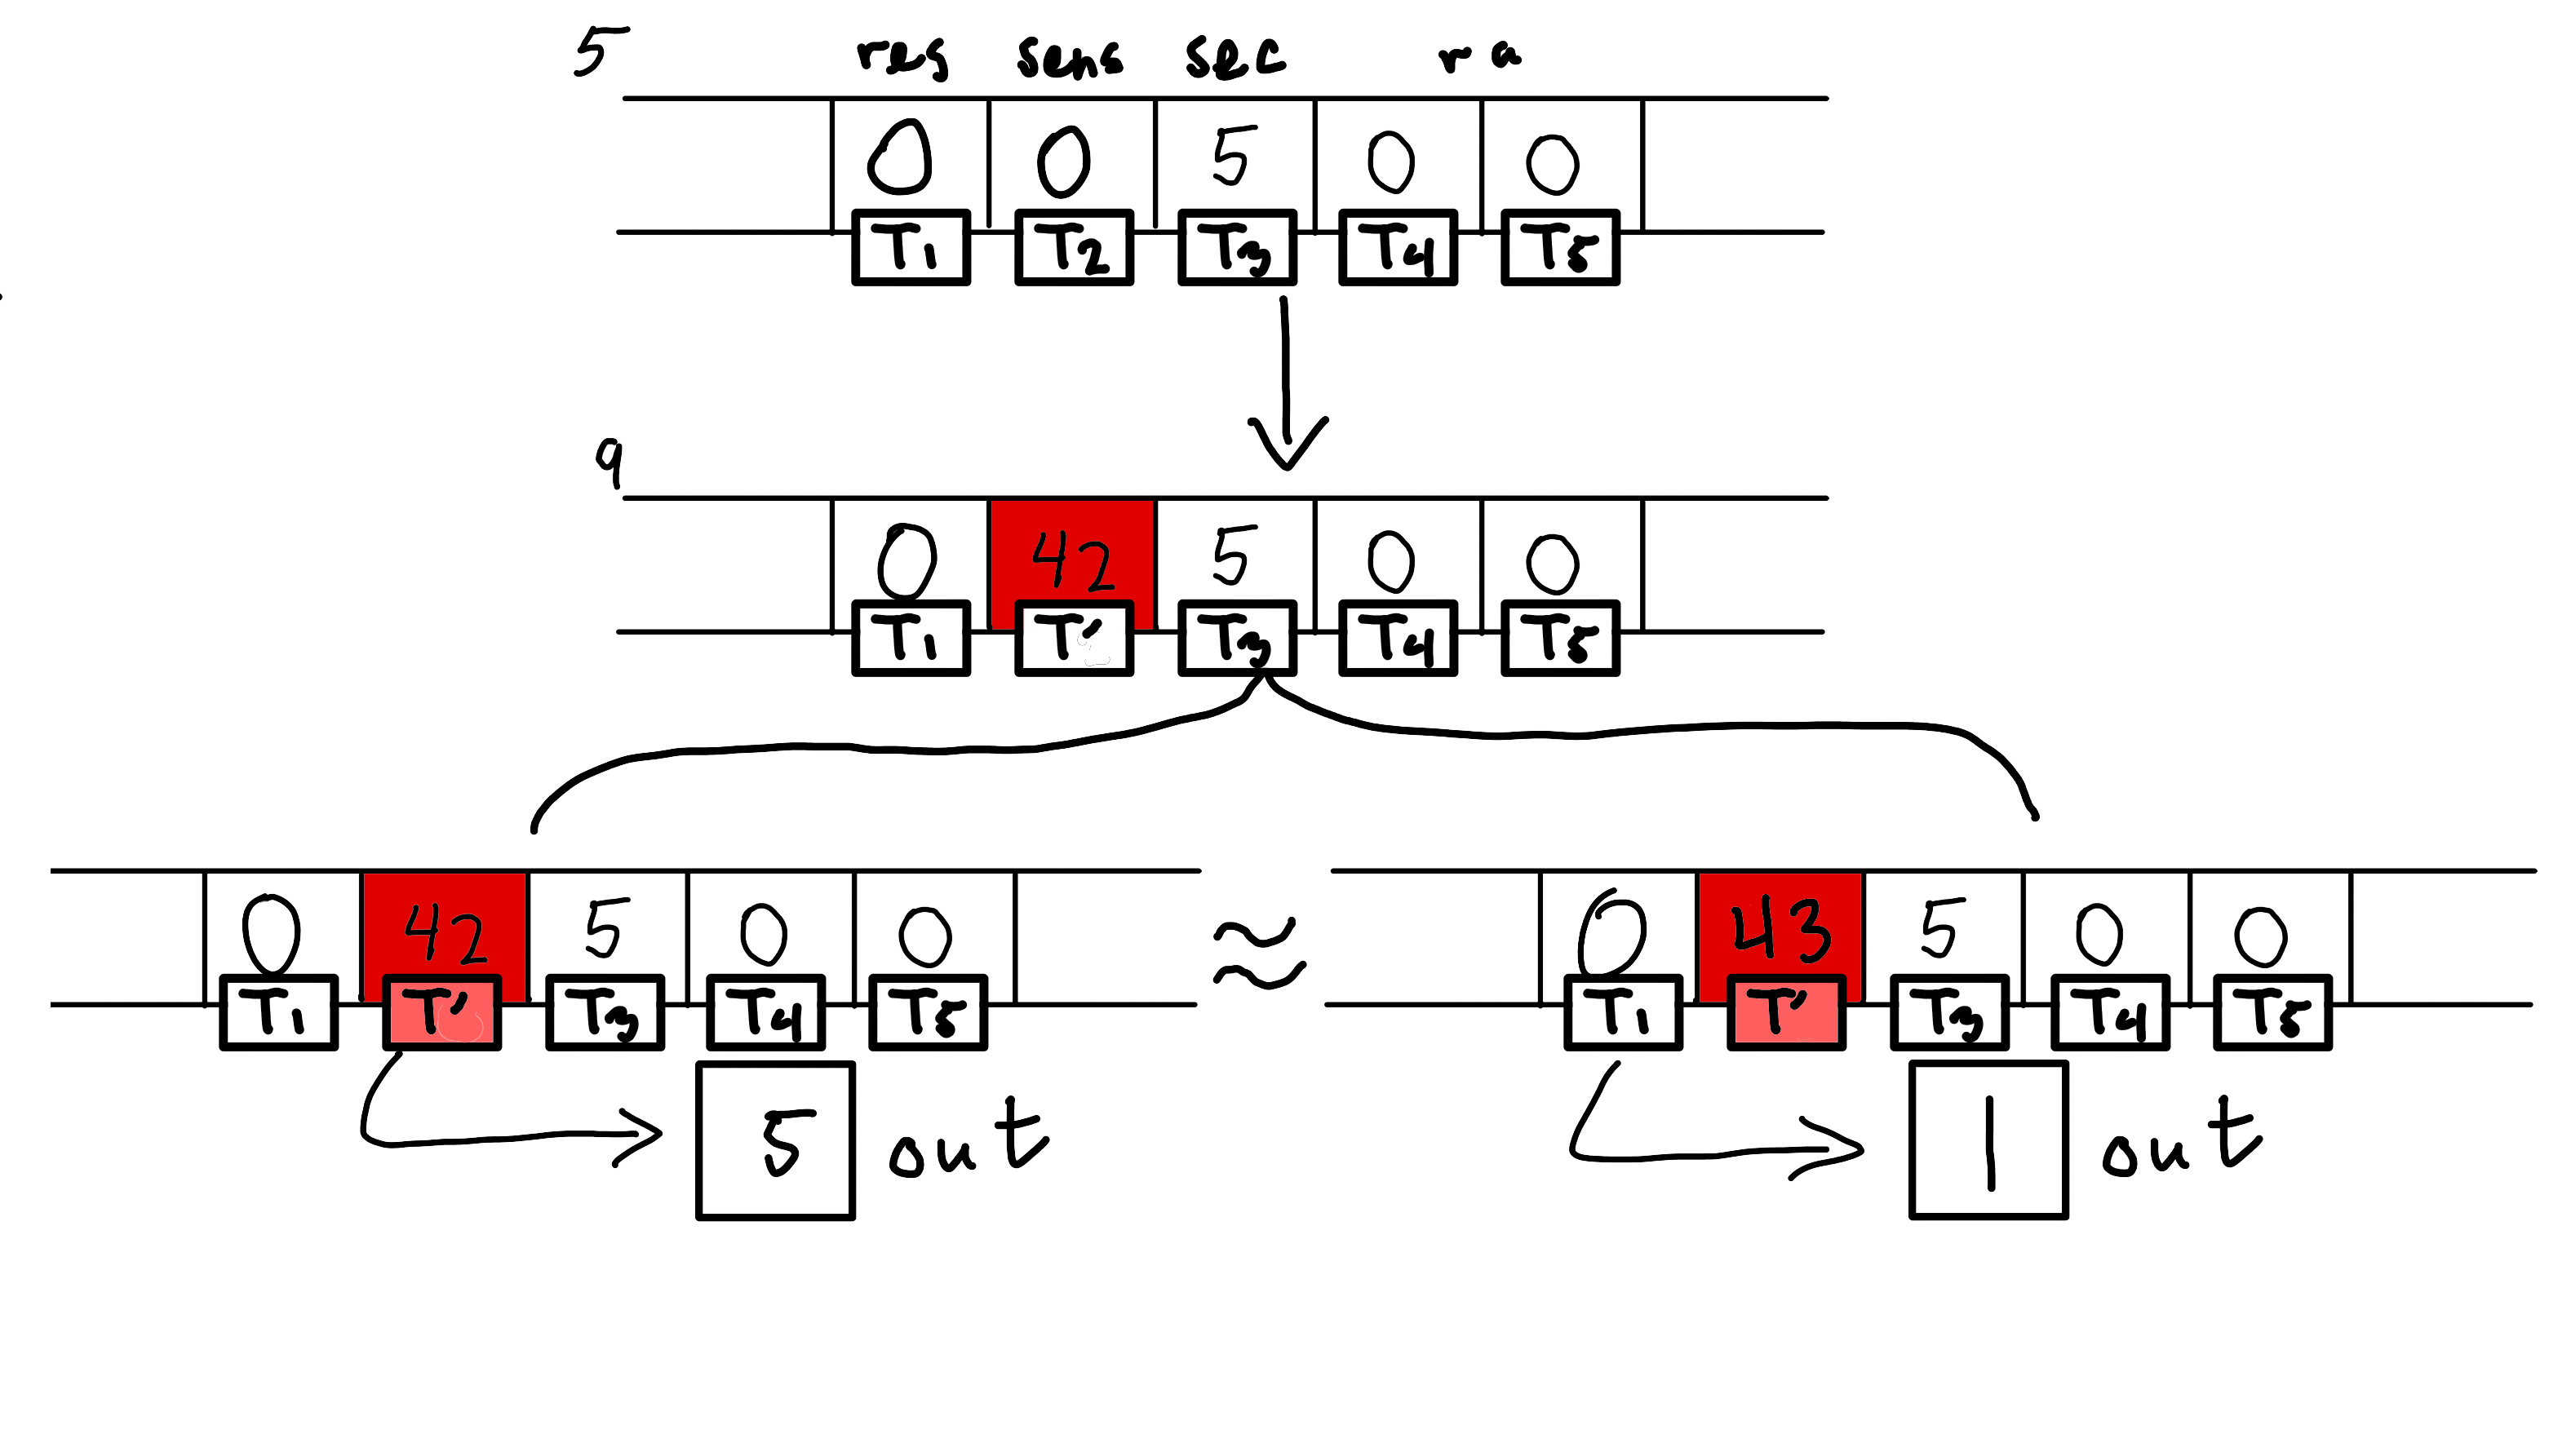
\includegraphics[width=\columnwidth]{variants.png}
  \caption{Integrity Violation\apt{Needs a machine-drawn version, as do the rest.}}
  \label{fig:variant}
\end{figure}

In our example setting, the observation trace consists of the sequence
of values written to {\tt out}.
The example in Figure \ref{subfig:integrity} modifies the value of {\tt sensitive},
which is \(\sealed\). Figure \ref{fig:variant} shows the state just after the call at step 5,
assuming that {\tt sec} is 5. Similar to WBCF, we will define
\(\intProp\) as a predicate on states that holds if
all relevant sealed addresses in \(\mach\) are the same as after step 5.
We once again require that \(\intProp\) hold on the state following the matching return,
which is reached by step 9. Here {\tt sensitive} has obviously changed, but is it relevant?
Consider a variant state in which {\tt sensitive} has any other value, arbitrarily
choosing 43 (and keeping its tag, \(t_2'\), unchanged.) As execution continues after the return
from the original state, it passes the {\tt if}-test on {\tt sensitive}, whereas the execution
from the variant does not, resulting in differing outputs. Therefore {\tt sensitive} \emph{is} relevant,
so \(\intProp\) does not hold, and integrity has indeed been violated.

\paragraph*{Caller Confidentiality}

We treat confidentiality as a form of non-interference as well: the confidentiality of a caller
means that its callee's behavior is dependent only on publicly visible data,
not the caller's private state. This also requires that the callee initialize
memory before reading it.
As we saw in the examples, we must consider both the observable events
that the callee produces during the call and the changes that the callee makes to the state that might
affect the caller after the callee returns.

Consider the state \(\mach\) after step 5, whose context is \((V_2,\sigma)\), with the attacker from
Figure \ref{subfig:direct}. We take a variant state over the set of element(s) that are
\(\sealed\) in \(V_2\) (see Figure \ref{fig:variant2}.)
            [TODO: fix figure to avoid varying the entire stack.]
If we take a trace of execution from each state until it returns,
the traces may differ, in this case outputting 5 (the original value of {\tt secret}) and
4 (its value in the variant) respectively. This is a violation of
{\it internal confidentiality} (formalized in \cref{tab:props}, line 3a).

\begin{figure}
  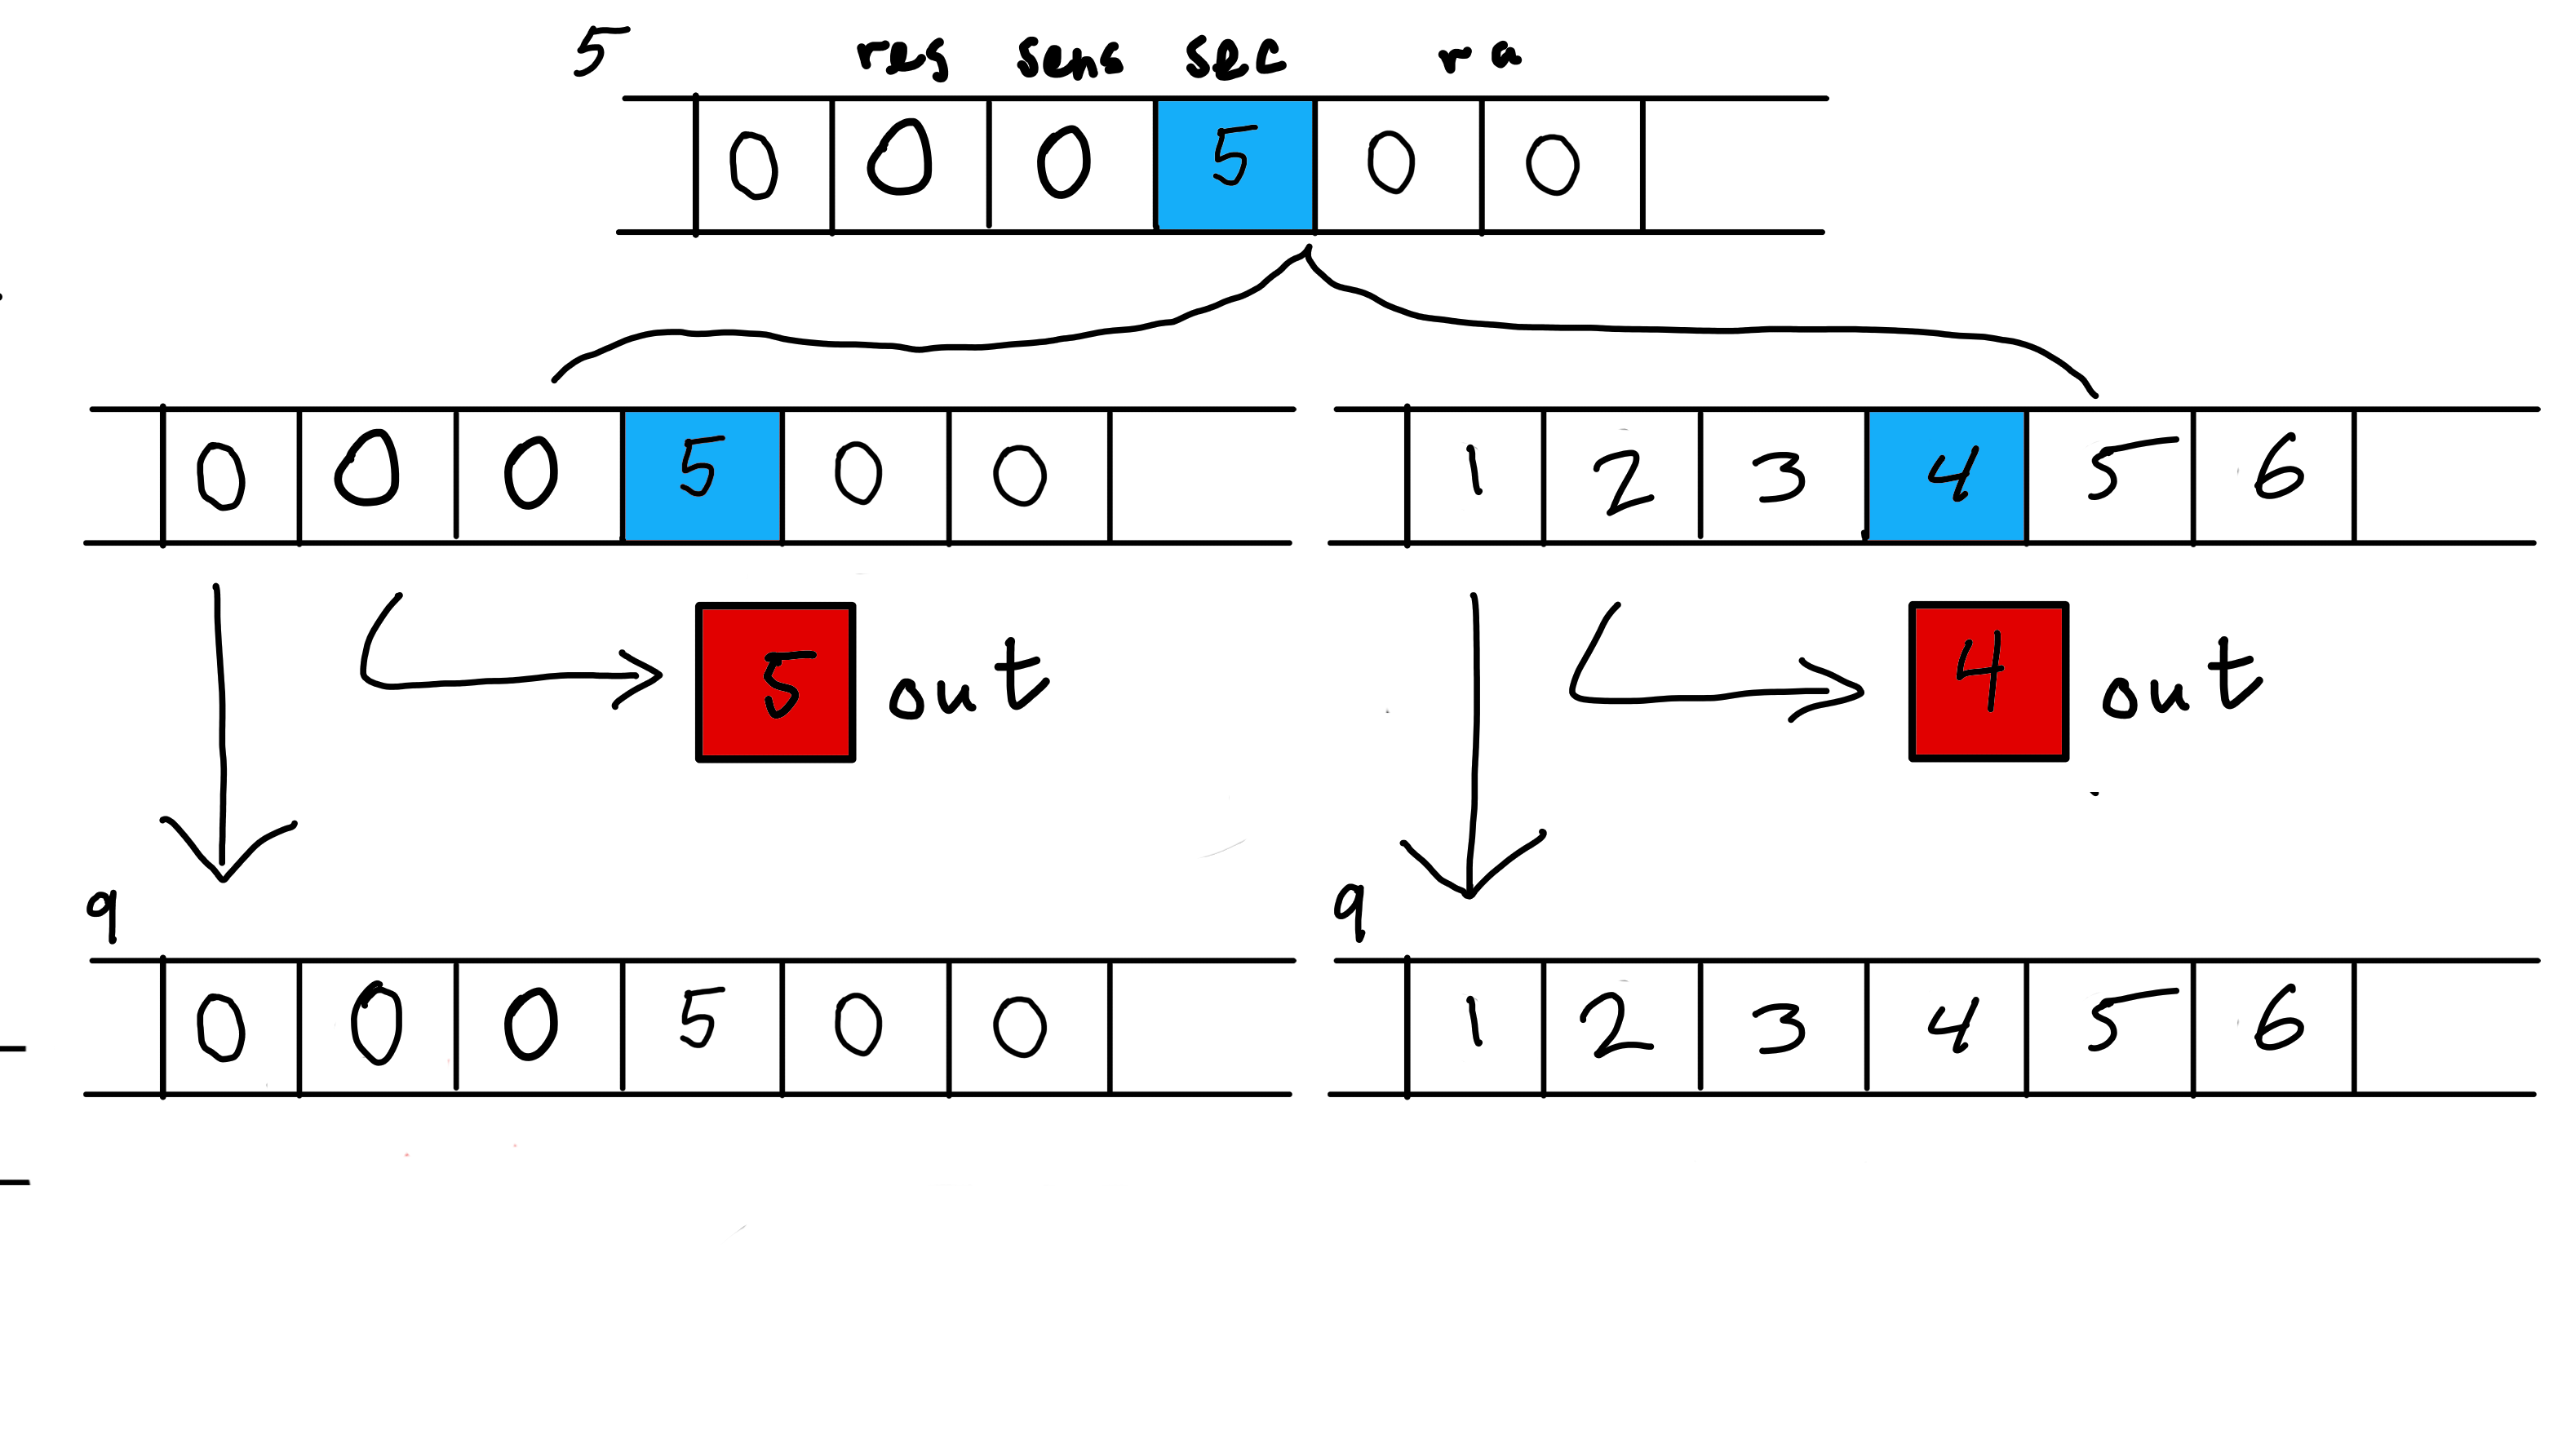
\includegraphics[width=\columnwidth]{variants2.png}
  \caption{Internal Confidentiality Violation}
  \label{fig:variant2}
\end{figure}

But, in Figure \ref{subfig:indirect}, we also saw an attacker that exfiltrated the secret
by reading it and then returning it, in a context where the caller would output the returned
value. Figure \ref{fig:variant3} shows the behavior of the same variants under this attacker,
but in this case, there is no output during the call. Instead the value of {\tt secret} is
extracted and placed in {\tt a0}, the return value register. We wish to identify this as
a confidentiality violation, again by considering variants of the \(\sealed\)
elements in \(V_2\), but capturing the required property is subtle.

To illustrate the issues, note that {\tt f} has also stores a 0 below the stack pointer.
%
\begin{figure}
  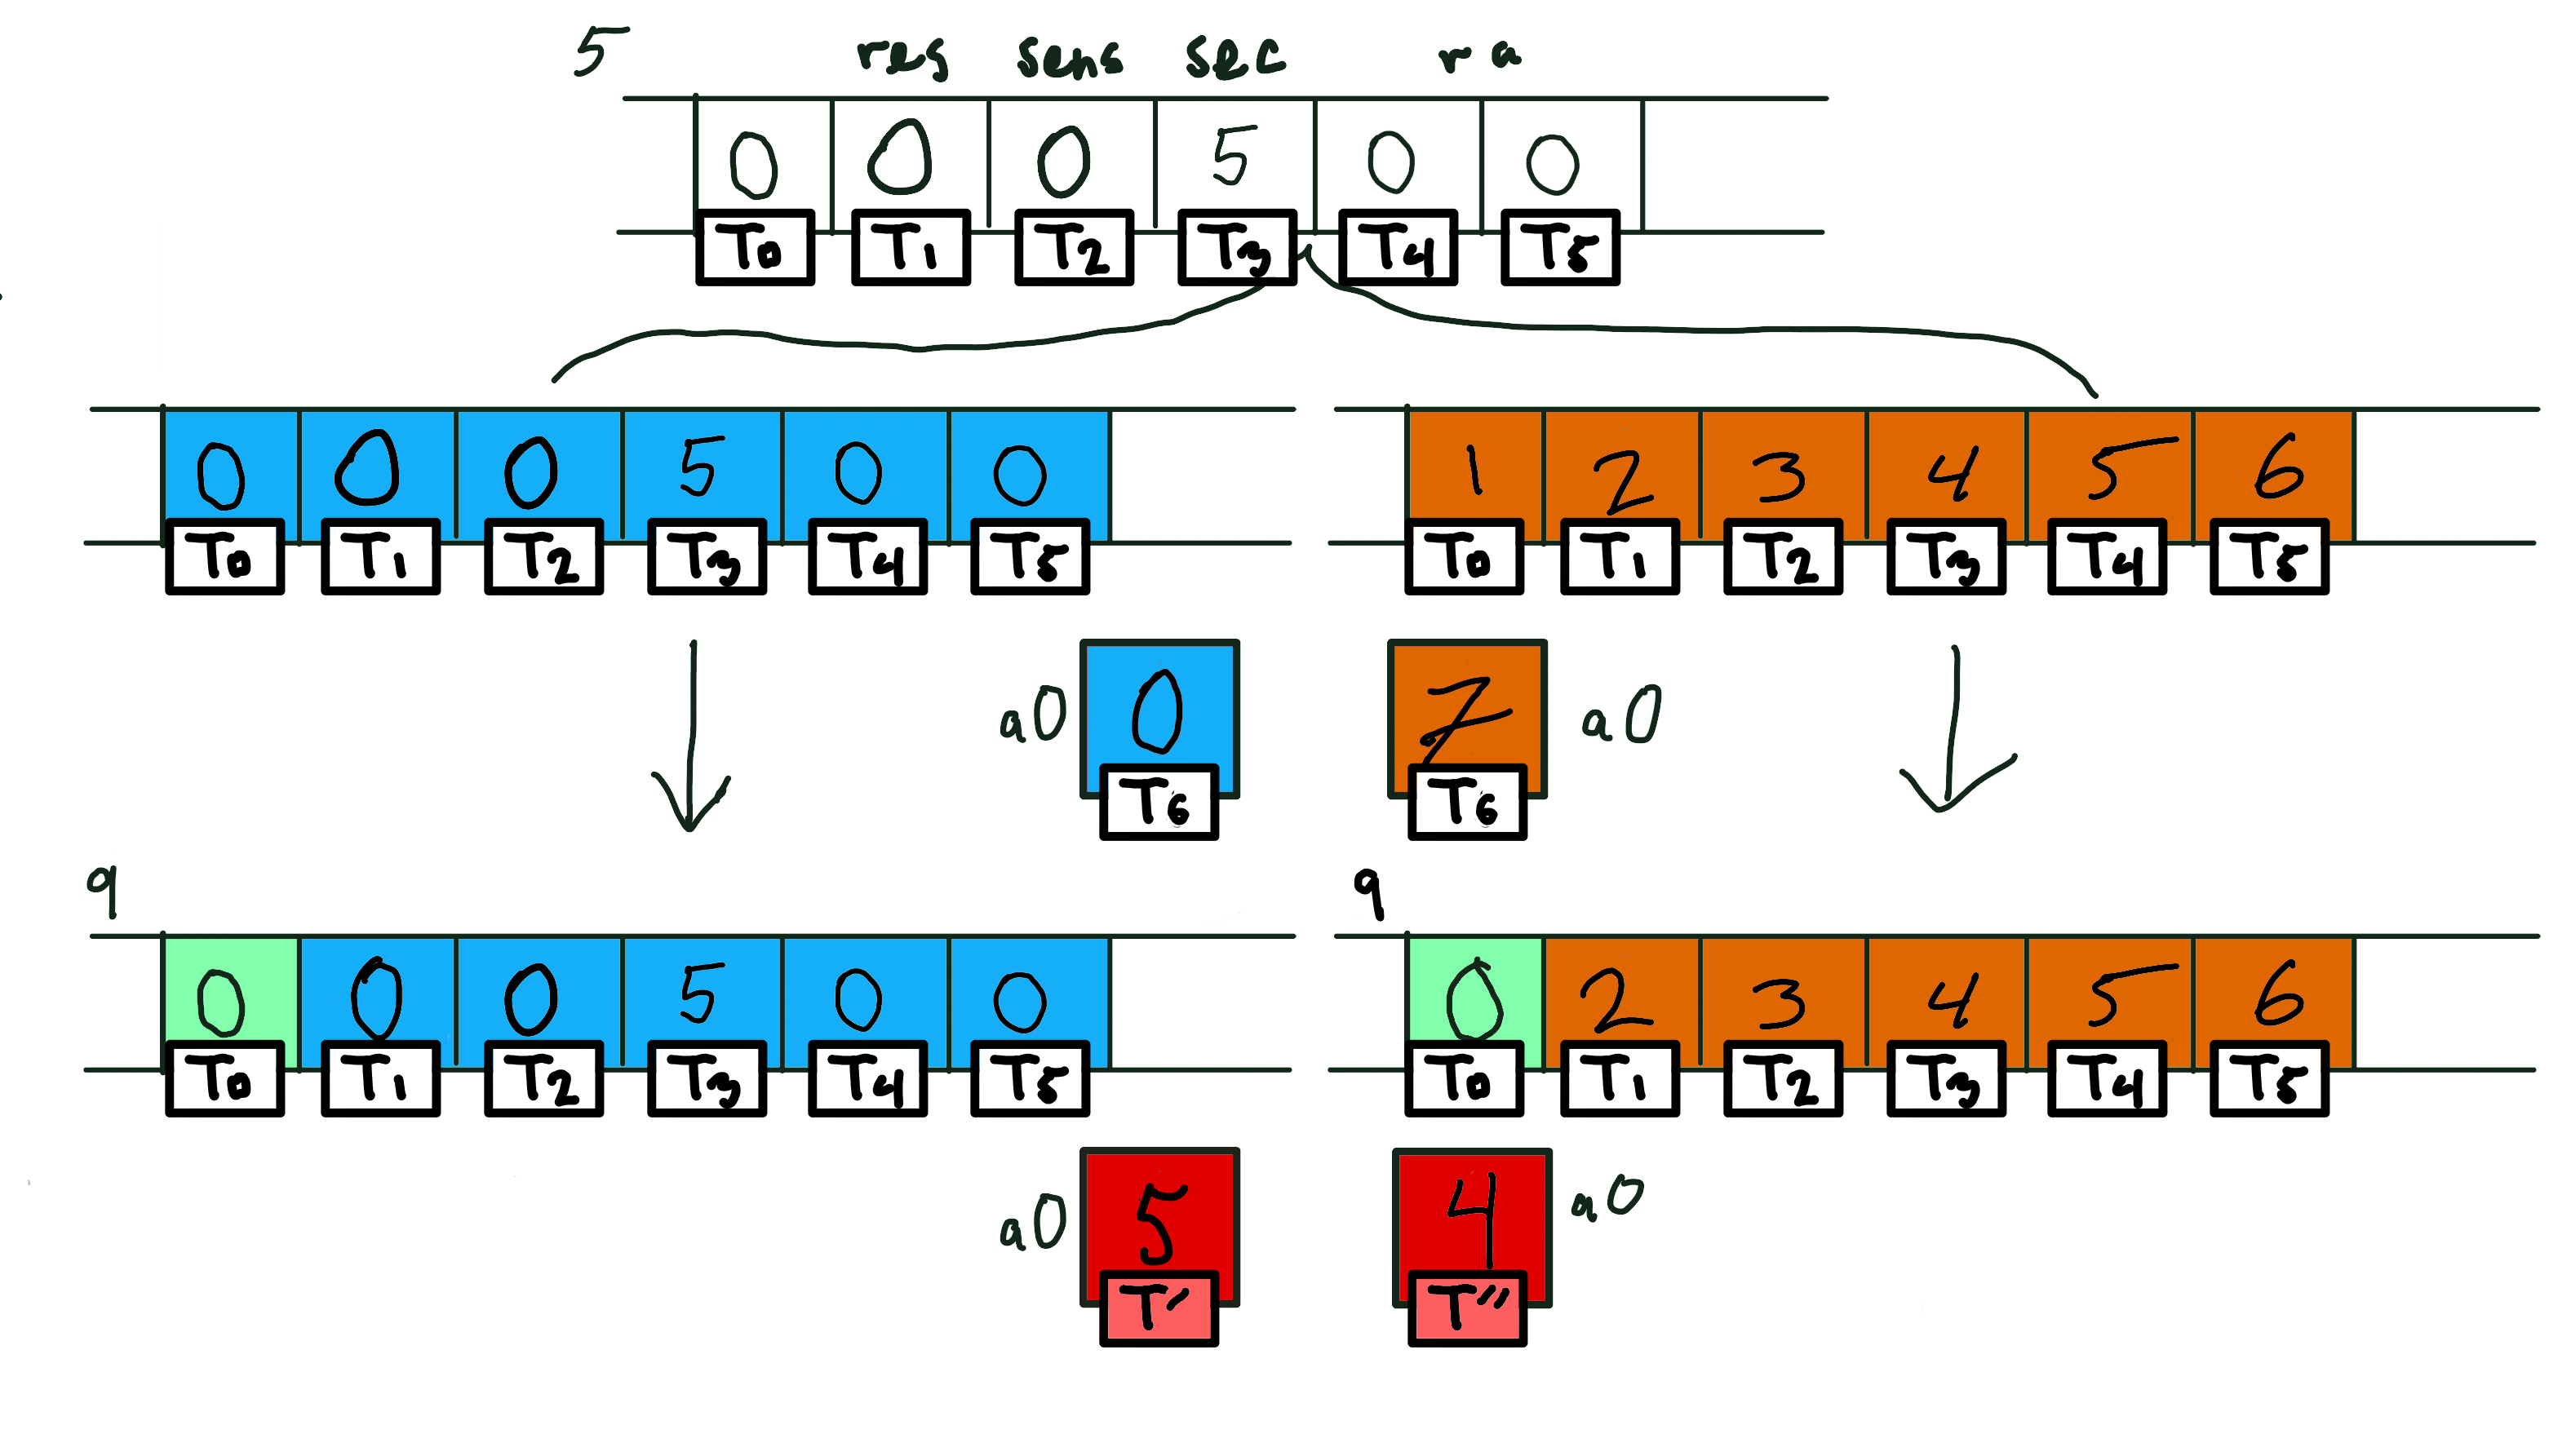
\includegraphics[width=\columnwidth]{variants3.png}
  \caption{Return-time Confidentiality Violation}
  \label{fig:variant3}
\end{figure}
%
Now consider three elements: the address \(\SP - 4\), the address \(\SP + 12\),
and the register {\tt a0}. The execution from the right-hand state to its return
has changed the value at \(\SP - 4\), but that value matches that of the
left-hand return. Therefore, the change does not represent a leak.

The return states disagree on the value of \(\SP + 12\). But in neither
case has that value changed since the original variants. So the difference is inherited from
the original variation, and does not represent a leak either. We do not continue executing the
variant state after return, so these values will not cause the caller to behave differently.

But in the case of {\tt a0}, the value has changed during the call (in both the original
and the variant, although only one of these would be necessary), and its final value
differs between the variants.
Therefore, it must depend on a secret (in fact, the variable {\tt secret}).
Unless {\tt a0} happens to be irrelevant, this is a violation of what
we term {\it return-time confidentiality} (formalized in \cref{tab:props}, line 3b).

Structurally, return-time confidentiality resembles integrity, but now dealing with
variants. We begin with a state immediately following
a call, \(\mach\). We consider an arbitrary variant state,
\(\nach\), which may vary any element that is \(\sealed\) or \(\unsealed\),
i.e., any element that is not used legitimately to pass arguments. Caller confidentiality
therefore can be thought of as the callee's insensitivity to elements in its initial state
that are not part of the caller-callee interface.

In place of a predicate, we define \(\confProp\) as a binary relation on states,
which holds on eventual return states \(\mach'\) and \(\nach'\)
iff all relevant elements that changed between \(\mach\) and \(\mach'\) or \(\nach\) and \(\nach'\)
are the same in \(\mach\) and \(\nach\). We then define
return-time confidentiality as holding if \(\confProp\) holds on the matching return states
from \(\mach\) and \(\nach\), respectively.

Finally, we define \emph{caller confidentiality} (\(\clrc\)) as the
combination of internal and return-time confidentiality (\cref{tab:props}, line 3).

\paragraph*{The Callee's Perspective}

We presented our initial example from the perspective of the caller, but a callee
may also have privilege that its caller lacks, and which must be protected from the
caller. Consider a function that makes a privileged system call to obtain a secret key,
and uses that key to perform a specific task. An untrustworthy or erroneous caller might
attempt to read the key out of the callee's memory after return, or to influence the callee
to cause it to misuse the key itself!
\apt{I believe this is the first point at which we suggest that our properties might be
  useful for enforcing (conventional) security goals --- which are definitely \emph{not}
  part of the usual targets for ``stack safety'' mechanisms. This needs a lot more foreshadowing!}

Where the caller's confidentiality and integrity are concerned with protecting specific,
identifiable state---the caller's stack frame---their callee equivalents are concerned
with enforcing the expected interface between caller and callee. Communication between
the principals should occur only through the state elements that are designated for the
purpose: those which we label \(\public\) and (in the presence of memory sharing) \(\object\).

The properties themselves correspond to their caller equivalents, inverted. \apt{Need at least their
  names, with references to formalizations in the table. And for the discussion in the next paragraph
  to make sense, we will need more than that. Especially because the formalization section now has
nothing to say!}

\paragraph*{The Hierarchy of Stack Safety}

\apt{This discussion should be merged with others on same topic, and maybe moved.}
The forms of stack safety described above can potentially be enforced separately
in various combinations. This is important, because
many existing enforcement mechanisms enforce only some of the stack safety
properties. Stricter enforcement may have greater performance impacts, leading to decisions
about trade-offs between different degrees of stack safety.

 \(\clec\) subsumes \(\clri\), and \(\clei\) subsumes
\(\clrc\), but integrity and confidentiality are in general orthogonal to each other
and to \(\wbcf\). Despite this, many enforcement techniques focus purely on
well-bracketed control flow. Stack canaries aim to prevent certain attacks on the return
address, and shadow stacks with protection (e.g. Return Address Defender \cite{Chiueh2001RAD})
to enforce it completely. Others combine this protection with some degree of memory protection,
chiefly focusing on integrity.

\section{Machine and Security Semantics, Formally}
\label{sec:machine}

\begin{figure}
  \begin{tabular}{| l | l | l |}
    \hline
    Set / & Names & Purpose \\
    Class & & \\
    \hline
    \(\mathit{CLR}\) / & {\tt t0} -- {\tt t6} & Caller-saved temps \\
    \(\unsealed\) & {\tt a0} -- {\tt a1} & Caller-saved args / return vals \\
    & {\tt a2} -- {\tt a7} & Caller-saved args \\
    & {\tt ra} & Return Address \\
    \hline
    \(\mathit{CLE}\) / & {\tt s0} -- {\tt s11} & Callee-saved \\
    \(\sealed\) & {\tt sp} & Stack Pointer \\
    \hline
    \(\mathit{PUBLIC}\) / & {\tt gp} & Global Pointer  \\
    \(\public\) & {\tt tp} & Thread Pointer \\
    \hline
  \end{tabular}
  \caption{RISC-V integer register set}
  \label{fig:RISCVregs}
\end{figure}

The building blocks of a machine are {\em words} and {\em registers}.
Words are ranged over by \(\word\) and, when used as addresses, \(\addr\),
and are drawn from the set \(\WORDS\).
Registers in the set \(\REGS\) are ranged over by \(\reg\), with the stack pointer
given the special name \(\SP\);
some registers may be classified as caller-saved or callee-saved.
Along with the program counter, \(\PCname\), these are referred to as
{\em state elements} \(\component\) in the set \(\COMPONENTS ::= \PCname | \WORDS | \REGS\).

A {\em machine state} \(\mach \in \MACHS\) is a map from state elements to a set \(\mathcal{V}\) of
\emph{values},  with a step function \(\mach \xrightarrow{\bar{\psi},\obs} \mach'\).
Each value \(v\) contains a \emph{payload} word, written \(|v|\).
The details of value structure depend on the specific machine being modelled;
intuitively, the payload represents the part of the value that is relevant to
the behavior of the basic machine, while the rest of the value may contain
information relevant to a hardware enforcement mechanism (such as a tag).
We write \(\mach[\component]\) to denote the value of \(\mach\) at
\(\component\)  and \(\mach[v]\) as shorthand for \(\mach[|v|]\).

Security classes are ranged over by \(l \in \{\public, \object, \sealed, \unsealed\}\).
For some security class \(l\), we write \(l(V)\)
to denote the set of elements \(\component\) such that \(V ~ \component = l\).
The {\it initial view} \(V_0\) maps all stack locations to \(\unsealed\),
all other locations to \(\public\), and registers based on which set they
belong to: \(\sealed\) for callee-saved, \(\unsealed\) for caller-saved, and \(\public\) otherwise.

A {\it context} is a pair of the current activation's view and
a list of views representing the call stack (pending inactive
principals), ranged over by \(\sigma\).

A view \(V\) maps elements to security classes, and a context consists of the
view of the active function together with a stack of inactive views.
The initial context is \(\context_0 = (V_0, \emplist)\).
%
\[\context \in \CONTEXTS ::= \mathit{VIEW \times list ~ VIEW}\]
%
We have described informally how the security context develops as the system performs
security-relevant operations. Formally, we combine each machine state with a context
to create a {\it combined state} \(s = (\mach,\context)\) and a lift the transition
transition \(\stepstounder{}\) on combined states, labeled with the same operations.
with each step, the context updates based on the function
\(Op : \MACHS \rightarrow \CONTEXTS \rightarrow \psi \rightarrow \CONTEXTS\).
Note that \(Op\) takes as its first argument the state {\it before} the step.
Since a single step might correspond to multiple operations, we apply
\(Op\) as many times as is needed.

\judgmenttwo{\(\mach \xrightarrow{\overline{\psi}} \mach', \obs \)}
            {\(\mathit{foldl} ~ (Op ~ \mach) ~ \context ~ \overline{\psi} = \context'\)}
            {\((\mach,\context) \stepstounder{\overline{\psi}} (\mach', \context', \obs)\)}

The definition of \(Op\) is most convenient to present decomposed into
rules for each operation. We have already seen the intuition behind the rules for
\(\mathbf{alloc}\), \(\mathbf{call}\), and \(\mathbf{ret}\).
For the machine described in the example, the \(Op\) rules would be those
found in \cref{fig:basicops}.

\begin{figure}
  \judgmentbr{\(\components = \mathit{range} ~ \SP ~ \mathit{off} ~ \mathit{sz} ~ \mach \cap
    \{\addr \mid V ~ \addr = \unsealed\}\)}
             {\(V' = V \llbracket \addr \mapsto \sealed \mid \addr \in \components \rrbracket\)}
             {\(Op ~ \mach ~ (\mathbf{alloc} ~ \mathbf{f} ~ \mathit{off, sz}) ~ (V,\sigma) = (V',\sigma)\)}
    %
    \judgmentbr{\(V' = V \llbracket \reg \mapsto \unsealed | \reg \in \mathit{CLR} \rrbracket
                 \llbracket \reg \mapsto \public | \reg \in \overline{\reg_{args}} \rrbracket\)}
               {\(V'' = V'\llbracket \addr \mapsto \sealed | V' ~ \addr = \object \land \addr \not \in (\mathit{passed} ~ \overline{sa} ~ \mach) \rrbracket\)}
               {\(Op ~ \mach ~ (\mathbf{call} ~ \addr_{target} ~ \overline{\reg_{args}} ~ \overline{sa})
                 ~ (V,\sigma) = (V'',V::\sigma)\)}
    %
    \judgment{\(\sigma = (V,\addr_{ret},\addr_{sp})::\sigma'\)}
             {\(Op ~ \mach ~ \mathbf{return} ~ (\_, \sigma) = (V, \sigma)\)}
  \caption{Basic Operations}
  \label{fig:basicops}
\end{figure}

\subsection{Events and Traces}
\label{sec:events}

We abstract over the events that can be observed in the system, defining them
only as a set \(\OBSS\) that contains at least the element \(\tau\), the silent
event. Other events might represent certain function calls (i.e., system calls)
or writes to special addresses representing mmapped regions.
A {\em trace} is a nonempty, finite or infinite sequence
of events, ranged over by \(\obsT\).
We use ``\(\notfinished{}{}\)'' to represent ``cons'' for traces, reserving ``::''
for list-cons.

We write the trace of execution from a state up to the first
state below depth \(d\) via the \(\hookrightarrow\) operator, defined coinductively.
When \(d = 0\), the trace will always be infinite. In this case we
omit \(d\) and just write \(\hookrightarrow s\).

\judgment{\(|\sigma| < d\)}
         {\(d \hookrightarrow (\mach,(V,\sigma)) = \tau\)}

\judgmentthree{\((\mach,(V,\sigma)) \stepstounder{} (\mach',\context',\obs)\)}
              {\(|\sigma| \geq d\)}
              {\(d \hookrightarrow (\mach',\context') = \obsT\)}
              {\(d \hookrightarrow (\mach,(V,\sigma)) = \notfinished{\obs}{\obsT}\)}


Two event traces $\obsT_1$ and $\obsT_2$ are {\em similar},
written \(\obsT_1 \eqsim \obsT_2\), if the sequence of non-silent events
is the same. That is, we compare up to deletion of \(\tau\) events.

\begin{minipage}{.4\columnwidth}
  \judgment{}{\(\obsT \eqsim \obsT\)}
\end{minipage}
\begin{minipage}{.4\columnwidth}
  \judgment{\(\obsT_1 \eqsim \obsT_2\)}
           {\(\notfinished{\obs}{\obsT_1} \eqsim \notfinished{\obs}{\obsT_2}\)}
\end{minipage}

\begin{minipage}{.4\columnwidth}
  \judgment{\(\obsT_1 \eqsim \obsT_2\)}
           {\(\notfinished{\tau}{\obsT_1} \eqsim \obsT_2\)}
\end{minipage}
\begin{minipage}{.4\columnwidth}
  \judgment{\(\obsT_1 \eqsim \obsT_2\)}
           {\(\obsT_1 \eqsim \notfinished{\tau}{\obsT_2}\)}
\end{minipage}

\section{Formal properties}
\label{sec:props}

Now we are ready to introduce the formal properties that define correctly enforced
security semantics. First, we must give a few prelimaries: the generation and comparison
of traces, variant states, and ``on-return'' assertions.

For a given system, we assume an compatibility equivalence relation \(\sim\) on values.
Two states are variants with respect to a set of elements \(\components\)
if they agree on the value of every element not in \(\components\) and
and have compatible values for every element in \(\components\).
Our notion of non-interference involves comparing the traces of such
\(\components\)-variants. We use this to define sets of irrelevant elements,
and secrets in general.

\definition Machine states \(\mach\) and \(\nach\) are {\em \(\components\)-variants},
written \(\mach \approx_\components \nach\), if, for
all \(\component \not \in \components\), \(\mach[\component] = \nach[\component]\)
and for all \(\component \in \components\), \(\mach[\component] \sim \nach[\component]\).

\definition An element set \(\components\) in state \((\mach,\context)\) contains
irrelevant values, written \((\mach,\context) \parallel \components\), if for all
\(\nach\) such that \(\mach \approx_{\components} \nach\),
\(\hookrightarrow (\mach,\context)  \eqsim \hookrightarrow (\nach,\context)\).

\definition \(\Delta(\mach,\mach')\) is the set of elements \(\component\)
such that \(\mach[\component] \not = \mach'[\component]\).

\definition The {\em corrupted set} \(\bar{\Diamond}(\mach,\mach',\nach,\nach')\)
is the set \((\Delta(\mach,\mach') \cup \Delta(\nach,\nach')) \cap \Delta(\mach',\nach')\).

Conceptually, the corrupted set treats \(\mach\) and \(\nach\) as initial states whose
and \(\mach'\) and \(\nach'\) as their corresponding final states, such that any element
that has changed from its initial value but does not match between the final states
is considered to have propagated some varied data from the original pair.

Our ``on-return'' assertions are defined using a second-order logical operator
\(d \uparrow P\), pronounced ``\(P\) holds on return from depth \(d\),''
where \(P\) is a predicate on machine states. This is a coinductive relation
similar to ``weak until'' in temporal logic---it also holds if the program never
returns from depth \(d\).

\judgmenttwo[Returned]
            {\(|\sigma| < d\)}
            {\(P ~ \mach\)}
            {\((d \uparrow P) ~ (\mach, (V,\sigma))\)}

\judgmenttwobrlong[Step]
                  {\(|\sigma| \geq d\)}
                  {\((d \uparrow P) ~ (\mach', \context')\)}
                  {\((\mach, (V,\sigma)) \stepstounder{\overline{\psi}} (\mach', \context',\obs)\)}
                  {\((d \uparrow P) ~ (\mach, (V,\sigma))\)}

Similarly, we give a binary equivalent for use in confidentiality. We define \(\Uparrow\) so that
\((\mach,\context) ~ (d \Uparrow R) ~ (\mach',\context')\) holds if \(R\) holds on the
first states that return from depth \(d\) after \((\mach,\context)\) and \((\mach',\context')\),
respectively. Once again, \(\Uparrow\) is coinductive.

\judgmentthree[Returned]
              {\(|\sigma_1| < d\)}
              {\(|\sigma_2| < d\)}
              {\(\mach_1 ~ R ~ \mach_2\)}
              {\((\mach_1,(V_1,\sigma_1)) ~ (d \Uparrow R) ~ (\mach_2,(V_2,\sigma_2))\)}

\judgmenttwobrlong[Left]
                  {\(|\sigma_1| \geq d\)}
                  {\((\mach_1,(V_1,\sigma_1)) \stepstounder{\overline{\psi}} (\mach_1',\context_1',\obs)\)}
                  {\((\mach_1',\context_1') ~ (d \Uparrow R) ~ (\mach_2,(V_2,\sigma_2))\)}
                  {\((\mach_1,(V_1,\sigma_1)) ~ (d \Uparrow R) ~ (\mach_2,(V_2,\sigma_2))\)}

\judgmenttwobrlong[Right]
                  {\(|\sigma_2| \geq d\)}
                  {\((\mach_2,(V_2,\sigma_2)) \stepstounder{\overline{\psi}} (\mach_2',\context_2',\obs)\)}
                  {\((\mach_1,(V_1,\sigma_1)) ~ (d \Uparrow R) ~ (\mach_2,\context_2')\)}
                  {\((\mach_1,(V_1,\sigma_1)) ~ (d \Uparrow R) ~ (\mach_2,(V_2,\sigma_2))\)}

Finally, we can define our core properties. They can be found in \cref{tab:props},
arranged to show their commonalities and distinctions. Each definition gives a criterion
quantified over states \(s\) that immediately follow call (or tail-call) steps.
If an execution can reach a state \(s'\) such that \(s' \stepstounder{\overline{\psi}} s\)
where \(\mathbf{call} ~ \addr ~ \overline{\reg} \in \bar{\psi}\), then \(s\) is the target
of a call. Likewise, if \(\mathbf{tailcall} ~ \addr ~ \overline{\reg} \in \bar{\psi}\), then
\(s\) is the target of a tailcall. As a shorthand, we write that each property is defined
by a criterion that must hold ``for all (tail)call targets \(s\).'

\(\wbcf\), \(\clri\), and \(\clec\) are each straightforward: they define predicates that must
hold on return from the call. \(\clrc\) and \(\clei\) both compare the execution of the
call state with that of a variant state, and are concerned with both their internal and
their return-time behavior. So, for some \(\nach\) that is an appropriate variant,
all states must fulfill an ``internal'' clause that their traces are similar,
and a ``return-time'' clause, that any potentially corrupted memory at their returns
is irrelevant.

\begin{table*}[h]
  \setlength{\tabcolsep}{1pt}
  \center
  \begin{tabular}{l r l l l}
    \rowcolor{black!20}
    1
    & \(\wbcf \triangleq\) & \(|\sigma| \uparrow \ret\)
    & \(\textnormal{ where } \ret ~ \mach' \textnormal{ iff }\)
    \(\mach'[\SP] = \mach[\SP] \land \mach'[\PCname] = \mach[\PCname]+4\)
%    & \(\textnormal{ when } (\mach,(V,\sigma)) \textnormal{ is called}\) \\
    & \(\textnormal{ for all call targets } (\mach,(V,\sigma))\) \\
    %
    \rowcolor{black!10}
    2
    & \(\clri \triangleq\) & \((|\sigma| \uparrow \intProp) ~ (\mach,(V,\sigma))\)
    & \(\textnormal{ where } \intProp ~ \mach' \textnormal{ iff }
    \mach' \parallel \sealed(V) \cap \Delta(\mach,\mach')\)
%    & \(\textnormal{ when } (\mach,(V,\sigma)) \textnormal{ is called}\) \\
    & \(\textnormal{ for all call targets } (\mach,(V,\sigma))\) \\
    %
    \rowcolor{black!20}
    3
    & \(\clrc \triangleq\) & \(\forall \nach \textnormal{ s.t. } \mach \approx_{\components} \nach,\)
    & \(\textnormal{ where } \components = \sealed(V)\)
%    & \(\textnormal{ when } (\mach,(V,\sigma)) \textnormal{ is (tail)called}\) \\
    & \(\textnormal{ for all (tail)call targets } (\mach,(V,\sigma))\) \\
    \rowcolor{black!20}
    3a & & \(|\sigma| \hookrightarrow (\mach,(V,\sigma)) \simeq |\sigma| \hookrightarrow (\nach,(V,\sigma))\) & & \\
    \rowcolor{black!20}
    3b & & \(\textnormal{ and } (\mach,(V,\sigma)) ~ (|\sigma| \Uparrow \confProp) ~ (\nach,(V,\sigma))\)
    & \(\textnormal{ where } (\mach' ~ \confProp ~ \nach') \textnormal{ iff }
    \mach' \parallel \bar{\Diamond}(\mach,\nach,\mach',\nach')\) & \\
    %
    \rowcolor{black!10}
    4
    & \(\clec \triangleq\) & \((|\sigma| \uparrow \cconfProp) ~ (\mach,(V,\sigma))\)
    & \(\textnormal{ where } \cconfProp ~ \mach' \textnormal{ iff }
    \mach' \parallel \Delta(\mach,\mach') - \components\)
%    & \(\textnormal{ when } (\mach,(V,\sigma)) \textnormal{ is (tail)called}\) \\
    & \(\textnormal{ for all (tail)call targets } (\mach,(V,\sigma))\) \\
    \rowcolor{black!10}
    & & & \(\textnormal{ where } \components = \public(V) \cup \object(V)\) & \\
    %
    \rowcolor{black!20}
    5
    & \(\clei \triangleq\) & \(\forall \nach \textnormal{ s.t. } \mach \approx_{\components} \nach,\)
    & \(\textnormal{ where } \components = \public(V) \cup \object(V)\)
%    & \(\textnormal{ when } (\mach,(V,\sigma)) \textnormal{ is (tail)called}\) \\
    & \(\textnormal{ for all (tail)call targets } (\mach,(V,\sigma))\) \\
   \rowcolor{black!20}
    5a & & \(|\sigma| \hookrightarrow (\mach,(V,\sigma)) \simeq |\sigma| \hookrightarrow (\nach,(V,\sigma))\) & & \\
    \rowcolor{black!20}
    5b & & \(\textnormal{ and } (\mach,(V,\sigma)) ~ (|\sigma| \Uparrow \confProp) ~ (\nach,(V,\sigma))\)
    & \(\textnormal{ where } (\mach' ~ \cintProp ~ \nach') \textnormal{ iff }
    \mach' \parallel \bar{\Diamond}(\mach,\nach,\mach',\nach')\) & \\
  \end{tabular}
  \caption{Properties}
  \label{tab:props}
\end{table*}

\section{Expanding the Machine}

The system we've modeled so far has been very simple, but our properties
support an important dimension of generality: adding features. We will now
briefly introduce the features of our primary testing machine.

The full machine defines additional operations, and extends some of the old ones.
We add a field \(\overline{sa}\) to the \(\mathbf{call}\) operation: a set of
triples of a register \(\reg\), a base offset \(\mathit{off}\), and a size \(sz\), denoting
that the object at the offset \(\mathit{off}\) from \(\reg\) is to be passed as an argument.
The new \(\mathbf{tailcall}\) operation has the same fields, but deals with tail-call
optimizations in which the callee will reuse the caller's stack. The \(\mathbf{alloc}\) operation
gains a boolen flag indicating whether the allocation is to be public, accessible to
all functions until deallocated. The rules are given in \cref{fig:advops}; the
rules in \cref{fig:basicops} can be recaptured by instantiating
\(\mathbf{call}\) with \(\overline{sa}\) as the empty set, and \(\mathbf{alloc}\)
with \(\mathbf{f}\).

\subsection{Sharing Stack Memory}
In our examples, we have presented a vision of stack safety in which
the interface between caller and callee is in the registers that pass
arguments and return values. This is frequently not the case in a realistic
setting. Arguments may be passed on the stack due to being spilled, as an implementation
of variadic arguments, or because they are reference objects that inherently have
pass-by-reference semantics. The caller may also take the address of a local object and
pass that as a pointer to its callee.

We refine our call operation to make use of the information that we have about
which memory contain arguments, \(\overline{sa}\). \(\overline{sa}\) is a set of
triples of a register, an offset from the value of that register, and a size.
We first define the helpful set \(\mathit{passed} ~ \overline{sa} ~ \mach\),
then extend the call operation to keep all objects in \(\mathit{passed}\) marked
as \(\object\) and seal everything else (\cref{sfig:stkargs}).

In this mechanism, we can describe an argument being passed by their relative address
with the operation \(\mathbf{call} ~ \dots ~ (\SP, \mathit{off}, \mathit{sz})\).
In the case of pass-by-reference semantics, if the compiler designates register
\(\reg\) as holding the reference, then the operations is
\(\mathbf{call} ~ \dots ~ (\reg, 0, \mathit{sz})\).

In both cases, the immediate callee retains access to the passed object, but future
callees will not---unless the object is passed-by-reference further down the stack.
On the other hand, in the case of a caller explicitly taking the address of an
object and passing it as a pointer, we have no way obvious way to limit the scope
of such sharing. 

Our primary machine treats this scenario as the caller allocating a ``public''
object that can be accessed by anyone until it's deallocated. We extend the
\(\mathbf{alloc}\) operation with a boolean flag, where {\bf t} indicates
that the allocation is public, and {\bf f} is private.
In the likely event that the space for multiple objects is allocated in a single step,
that step can make multiple allocation operations, each labeled appropriately.
Allocating public objects affects the call stack very similarly to private ones,
but instead of labeling them \(\object\) they become \(\public\), so they are
never sealed at a call (\cref{sfig:publicalloc}).

\begin{figure*}
  \begin{subfigure}{0.4\textwidth}
    \[\mathit{range} ~ \reg ~ \mathit{off} ~ \mathit{sz} ~ \mach \triangleq
    \{\mach[\reg]+i | \mathit{off} \leq i < \mathit{off+sz}\}\]
    
    \judgmentbr{\(\components = \mathit{range} ~ \SP ~ \mathit{off} ~ \mathit{sz} ~ \mach \cap
                 \{\addr \mid V ~ \addr = \unsealed\}\)}
               {\(V' = V \llbracket \addr \mapsto \sealed \mid \addr \in \components \rrbracket\)}
               {\(Op ~ \mach ~ (\mathbf{alloc} ~ \mathbf{f} ~ \mathit{off, sz}) ~ (V,\sigma) = (V',\sigma)\)}
             
    \judgmentbr{\(\components = \mathit{range} ~ \SP ~ \mathit{off} ~ \mathit{sz} ~ \mach \cap
                 \{\addr \mid V ~ \addr = \unsealed\}\)}
               {\(V' = V \llbracket \addr \mapsto \public \mid \addr \in \components \rrbracket\)}
               {\(Op ~ \mach ~ (\mathbf{alloc} ~ \mathbf{t} ~ \mathit{off, sz}) ~ (V,\sigma) = (V',\sigma)\)}
    %
    \judgmentbr{\(b = \mach[\SP] + \mathit{off}\)}
               {\(V' = V \llbracket \addr \mapsto \unsealed |
                 b \leq a < b+\mathit{sz} \land V ~ \addr = \object \rrbracket\)}
               {\(Op ~ \mach ~ (\mathbf{dealloc} ~ \mathit{off, sz}) ~ (V,\sigma) = (V',\sigma)\)}

    \caption{Memory Allocation}
    \label{sfig:publicalloc}
  \end{subfigure}
  \begin{subfigure}{0.6\textwidth}
    %
    \[\mathit{passed} ~ \overline{sa} ~ \mach = \bigcup_{(\reg,\mathit{off},\mathit{sz}) \in \overline{sa}}
    \mathit{range} ~ \reg ~ \mathit{off} ~ \mathit{sz} ~ \mach\]
    %
    \judgmentbr{\(V' = V \llbracket \reg \mapsto \unsealed | \reg \in \mathit{CLR} \rrbracket
                 \llbracket \reg \mapsto \public | \reg \in \overline{\reg_{args}} \rrbracket\)}
               {\(V'' = V'\llbracket \addr \mapsto \sealed | V' ~ \addr = \object \land \addr \not \in (\mathit{passed} ~ \overline{sa} ~ \mach) \rrbracket\)}
               {\(Op ~ \mach ~ (\mathbf{call} ~ \addr_{target} ~ \overline{\reg_{args}} ~ \overline{sa})
                 ~ (V,\sigma) = (V'',V::\sigma)\)}
    %
    \judgmentbr{\(V' = V \llbracket \reg \mapsto \unsealed | \reg \in \mathit{CLR} \rrbracket
                 \llbracket \reg \mapsto \public | \reg \in \overline{\reg_{args}} \rrbracket\)}
               {\(V'' = V'\llbracket \addr \mapsto \unsealed | V' ~ \addr = \object \land \addr \not \in (\mathit{passed} ~ \overline{sa} ~ \mach) \rrbracket\)}
               {\(Op ~ \mach ~ (\mathbf{tailcall} ~ \addr_{target} ~ \overline{\reg_{args}} ~ \overline{sa})
                 ~ (V,\sigma) = (V',\sigma)\)}
    %
    \judgment{\(\sigma = (V,\addr_{ret},\addr_{sp})::\sigma'\)}
             {\(Op ~ \mach ~ \mathbf{return} ~ (\_, \sigma) = (V, \sigma)\)}

    \caption{Calls with Argument Passing on the Stack}
    \label{sfig:stkargs}
  \end{subfigure}
  \caption{Operations}
  \label{fig:advops}
\end{figure*}

\subsection{Tail Calls}

The operation rule for a tailcall is similar to that for a normal call.
We do not push the caller's view onto the stack,
but replace it outright. This means that a tailcall does not increase the size of
the call stack, and therefore for purposes of our properties, all tailcalls will
be considered to return simultaneously when the eventual {\bf return} operation
pops the top of the stack.

Since the caller will not be returned to, it does not need integrity, though
it should still enjoy confidentiality. We set its frame to \(\unsealed\) rather
than \(\sealed\) to express this. Of course, some objects may be passed as arguments
in place, easily modeled by including them in \(\overline{sa}\). More sophisticated
behaviors may require sequences of {\bf dealloc}, {\bf tailcall}, then {\bf alloc}.

\section{Validation through Random Testing}
\label{sec:testing}

[TODO: this is still last submission's test. Kept here to get a sense of length.]

There are several ways to evaluate whether an enforcement mechanism enforces
stack safety properties. Ideally such validation would be done through formal proof over
the semantics of the enforcement-augmented machine.
However, while there are no fundamental barriers to producing such a proof,
it would be considerable work to carry out for a full ISA like RISC-V and
complex enforcement mechanism like the Depth Isolation micro-policy.
We therefore choose to validate the micro-policy of \cref{sec:enforcement} by
systematically \emph{testing} that it satisfies our properties.
This focus on testing is better aligned with our immediate
goal of evaluating real enforcement mechanisms for real machine architectures.
Formal proof remains future work.

We validate the micro-policy of the previous section by
systematically testing that it satisfies eager stack integrity and
confidentiality. We use a Coq specification of the RISC-V
architecture~\cite{Bourgeat2021AMF},
and extend it with a runtime monitor implementing a stack safety
micro-policy. We chose the Coq proof assistant as the setting for our implementation
to ensure that our coinductive trace definitions are well-formed, to reason about
them, and to leverage the power of the QuickChick property-based testing framework~\cite{Pierce:SF4}.

To use QuickChick, we build random test-case generators that produce
(1) an initial RISC-V machine state, including most notably
  the program to be executed;
(2)
  an initial policy state, tagging instructions corresponding to
  blessed call or return sequences appropriately, while marking
  all potential stack locations as $\tagNoDepth$; and
(3)
  a map from instructions to lists of their operations in the security semantics.

To write such generators we build on the work of
Hri\c{t}cu et al. \cite{TestingNI:ICFP, DBLP:journals/jfp/HritcuLSADHPV16}, which
introduced {\em generation by execution} to produce progams that lead
machines towards interesting behaviors. We extend the technique by tracking
control flow information so that programs will usually---but not always---return to their call sites.

%\paragraph*{Generators}
%
% Generation by
%execution receives as an input a partially instantiated machine state
%and attempts to generate an instruction (or a sequence of instructions
%such as a blessed sequence) that makes sense locally (e.g., jumps go
%to a potentially valid code location and loads read from a
%potentially valid stack location). Then we step the machine and repeat
%the process until we generate or execute some target number of
%instructions, or reach a point where the machine cannot step
%any more.
%
%We extend this technique to keep track of the control flow behavior of
%the program being generated: each time a call or return sequence is
%generated, we ensure that the appropriate policy tags and code
%annotations are set for the entry or return points.% At the same time,
%%we allow the generation to sometimes relax constraints,
%%introducing potentially ill-formed flows: this causes our programs
%%to failstop when executed in conjunction with the policy monitor,
%%but also allows for revealing errors in our setup.\apt{??}
%
We need to extend typical testing schemes further to handle the nested
nature of confidentiality: rather than just generating two
initial machines that are variants of one another and letting them
execute to test for noninterference, we generate a new variant
{\em every time a call is made} and check confidentiality for the
subtrace produced from that variant state until its corresponding
return. As a result, a ``single'' confidentiality test compactly
checks multiple nested calls.

Our primary testing targets are the eager {\em Depth Isolation}
and the {\em Lazy Per-Activation Tagging and Clearing} micro-policies.
We test the former against stepwise integrity and confidentiality, and
the latter against their observational counterparts.

To ensure the effectiveness of testing against our formal properties, we
use {\em mutation testing}~\cite{JiaH11}. In mutation testing, we inject errors
(mutations) in a program that should cause the property of interest (here,
stack safety) to fail, and ensure that the testing framework can find
them. The bugs we use for our evaluation are either artificially generated
by us (deliberately weakening the micro-policy in ways that we expect
should break its guarantees), or actual bugs that we discovered through
testing our implementation. We elaborate on some such bugs below.

For example, when loading from a stack location, {\em Depth Isolation}
needs to enforce that the tag on the location being read
is $\tagStackDepth{n}$ for some number $n$ and that the tag of the
current $\PCname$ is $\tagPCDepth{n}$ for the same depth $n$. We can relax
that restriction by not checking the depth equality (row {\em
  LOAD\_NO\_CHECK\_DI}).

Similarly, when storing to a stack location, the correct micro-policy
needs to ensure that the tag on the memory location is either
$\tagNoDepth$ or has again the same depth as the current $\PCname$
tag. Relaxing that constraint causes violations to the integrity
property (row {\em STORE\_NO\_CHECK}).

\begin{table}[]
\centering
\begin{tabular}{c|c|c|c}
  Bug & Property Violated & MTTF (s) & Tests \\
  \hline
      {\em LOAD\_NO\_CHECK\_DI}  & Confidentiality & 24.2 & 13.3 \\
      {\em STORE\_NO\_CHECK} & Integrity & 26.9 & 26 \\
      {\em HEADER\_NO\_INIT} & Integrity & 69.5 & 76.3 \\
  \hline
  \hline
      {\em PER\_DEPTH\_TAG} & Obs. Integrity & 189.7 & 8342.5  \\
      {\em LOAD\_NO\_CHECK\_LT}  & Obs. Integrity & 23.5 & 12.0 \\
      {\em LOAD\_NO\_CHECK\_LT}  & Confidentiality & 19.2 & 695.5 \\
      {\em STORE\_NO\_UPDATE} & Obs. Integrity & 70 & 80.6  \\
      {\em STORE\_NO\_UPDATE} & Confidentiality & 4.9 & 88.5 \\
  \hline
\end{tabular}
\vspace*{1em}
\caption{MTTF for finding bugs in erroneous policy enforcement mechanisms}
\vspace*{-2em}
\label{tab:bug-table}
\end{table}

The mean-time-to-failure (MTTF) and average number of tests for various bugs can be found in
Table~\ref{tab:bug-table}, along with the average number of tests
it took to find the failure. Experiments were run in a desktop
machine equipped with i7-4790K CPU @ 4.0GHz with 32GB RAM.

Naturally, testing also revealed a number of errors in our
implementation of the enforcement mechanism (the original was written in C++
and targeted ARM machine code;
%\bcp{right?}\leo{yeah}
we re-implemented it in Coq targeting RISC-V).  These errors range
from trivial typos to ones that require an intriguingly complex setup
to provoke.  The most interesting bug (included in the table as row
{\em HEADER\_NO\_INIT}) was that, on our first try, the blessed call
sequence %/policy combination\apt{??}
did not initialize all locations for the
newly allocated stack frame correctly, but left some of them as
$\tagNoDepth$. This allowed for a potential integrity violation, but
only if a rather complicated sequence of events occured.
The smallest counterexample requires calling a function {\tt f},
which fails to initialize some of its frame during the blessed sequence,
but writes into an uninitialized location $l$ later, treating \(l\) as outside
the stack. Then {\tt f} calls a further function {\tt g} (which should have
the effect of sealing $l$ for integrity purposes). {\tt g} attempts to write to $l$,
which is allowed because the enforcement mechanism still has
$l$ tagged as $\tagNoDepth$, but violates the integrity property on {\tt f}'s data.
%\sna{I believe what went wrong was that we were off-by-one in {\tt main}'s initialization,
%  and the write from {\tt f} was already a violation.}

As for lazy micro-policies and observational properties,
the original {\em Lazy Tagging and Clearing} micro-policy, implemented as {\em PER\_DEPTH\_TAG},
fails in testing, in cases where data is leaked between sequential calls.
To round out our mutation testing we also check {\em LOAD\_NO\_CHECK\_LT},
equivalent to its counterpart in depth isolation,
and a version where stores succeed but fail to propagate the PC tag, {\em STORE\_NO\_UPDATE}.
It turns out that {\em PER\_DEPTH\_TAG} is a comparatively subtle bug,
taking twice as long to catch as the next longest.

Our properties have allowed us to identify an enforcement mechanism as
not really stack safe, and to validate a possible fix.
Unfortunately, Lazy Per-activation Tagging and Clearing
puts severe pressure on the tag cache, so it may not be usable in practice.
However, we conjecture that no lazy scheme can be fully stack safe
without using unique per-activation identifiers.

\section{Future Work}
\label{sec:future}

From here, we see two natural ways to extend the work.
First, we should thoroughly evaluate
other enforcement mechanisms, especially Cheri-based capability
systems. Second, we can further demonstrate
the functionality of our definitions by using them to prove
the correctness of a programming logic with strengthened rules around calls and returns.

\paragraphx{Stack Safety in the Cheri Ecosystem}
%
There are several proposals around the use of Cheri capabilities to enforce stack safety,
including mechanisms that use the standard Cheri hardware (which includes local
capabilities) \cite{SkorstengaardLocal},
and others that propose entirely new types of capabilities, such as linear
\cite{SkorstengaardSTK}, uninitialized \cite{Georges+21}, lifetime
\cite{Tsampas+19}, and directed \cite{Georges22:TempsDesCerises} capabilities.
Of these, the last seems particularly promising for testing.
[TODO: more about this. (Rob's suggestion of citing Aina could go here.)]

\bibliographystyle{IEEEtran}
\bibliography{bcp.bib,local.bib}

\appendix

\subsection{Provenance, Capabilities, and Protecting Objects}
\label{app:ptr}

What if we want to express a finer-grained notion of safety, in which
stack objects are protected unless the function that owns them intentionally
passes a pointer to them? This can be thought of as a {\it capability}-based
notion of security. Capabilities are unforgeable tokens that grant access to
a region of memory, typically corresponding to valid pointers to that region.
So, in order to express such a property, we need our machine to carry some notion
of {\it pointer provenance}---a distinction between a pointer that is intended to
point to a given object, and non-pointer integers as well as pointers to other objects.

One such provenance model is Memarian et al.'s PVI \cite{}, in which pointers are
annotated with the identity of the object they first pointed to. This annotation is
propagated when the pointer is copied and when operations are performed on it---even
integer-only operations.

We can model this as a trio of additional security-relevant operations: one which
declares a register to contain a valid pointer, one which transmits the provenance
of a pointer from one element to another, and one which clears the provenance
(for instance, when a pointer is modified in place in a way that makes it invalid.)

In addition to the normal call stack, our security context will carry a map \(\rho\) from
elements to memory regions, represented as a base and a bound \(\context = (V, \sigma, \rho)\).
Existing operations are extended to keep the value of \(\rho\) the same, and the new operations
work as follows:

\judgmentbr[Promote]
           {\(\psi = \mathbf{promote} ~ \reg_{dst} ~ (\reg_{base},\mathit{off},\mathit{sz})\)}
           {\(\rho' = \rho[\reg_{dst} \mapsto \mathit{range} ~ \reg_{base} ~ \mathit{off} ~ \mathit{sz}]\)}
           {\(Op ~ \mach ~ \psi ~ (V,\sigma,\rho) = (V,\sigma,\rho')\)}

\judgmentbr[Propagate]
           {\(\psi = \mathbf{propagate} ~ \component_{src} ~ \component_{dst}\)}
           {\(\rho' = \rho[\component_{dst} \mapsto \rho[\component_{src}]]\)}
           {\(Op ~ \mach ~ \psi ~ (V,\sigma,\rho) = (V,\sigma,\rho')\)}

\judgment[Clear]
         {\(\psi = \mathbf{clear} ~ \component\)}
         {\(Op ~ \mach ~ \psi ~ (V,\sigma,\rho) = (V,\sigma,\rho[\component \mapsto \emptyset])\)}

We now have a notion of provenance, and must integrate it into the definition of
stack safety. We essentially generalize the above notion of passing: we will consider
a caller to have intentionally passed an object if that object is reachable by
a capability that has been passed to the callee. This includes capabilities passed
indirectly, by being stored in an object that is in turn passed. Formally, we call
this set \(\mathit{capped}\), and define it recursively:
%
\[\begin{split}
& \mathit{capped} ~ \components ~ \rho \triangleq \bigcup_{\component \in \components} \{\component\} \cup \mathit{capped} ~ \components' ~ \rho \textnormal{ where} \\
& \components' = \{\component' |\rho[\component] = (\mathit{base},\mathit{bound})
\land \mathit{base} \leq \component' < \mathit{bound}\} \\
\end{split}\]

We then tweak the call operation to seal only objects that are in \(\mathit{capped}\), or
the previously defined \(\mathit{passed}\).

\judgmentbrbrbr[]
               {\(\psi = \mathbf{call} ~ \addr_{target} ~ \overline{\reg_{args}} ~ \overline{sa}\)}
               {\(V' = V \llbracket \reg \mapsto \unsealed | \reg \in \mathit{CLR} \rrbracket
                 \llbracket \reg \mapsto \public | \reg \in \overline{\reg_{args}} \rrbracket\)}
               {\(\components = \{\addr | V' ~ \addr = \object \land \addr \not \in (\mathit{passed} ~ \overline{sa} ~ \mach) \cup (\mathit{capped} ~ \overline{\reg_{args}} ~ \rho) \}\)}
               {\(V'' = V'\llbracket \components \mapsto \sealed \rrbracket\)}
               {\(Op ~ \mach ~ \psi ~ (V,\sigma,\rho) =
                 (V'',V::\sigma,\rho)\)}

Note that we have a degree of monotonicity here. Once an object is sealed (because its
capability has not been passed to a callee), subsequent nested calls can never unseal it.
On the other hand, an object that is passed via a pointer may be passed on indefinitely.
              
\end{document}
